\documentclass[a4paper, 10pt]{article}
\usepackage[brazil]{babel}
\usepackage[utf8]{inputenc}
\usepackage[T1]{fontenc}
\usepackage{ae}
\usepackage[pdftex]{graphicx}
\usepackage{listings} %codigo
\usepackage{mips} 
\usepackage{nanoRisk} 
\usepackage{xcolor}
%\pagestyle{headings}
\usepackage{indentfirst}
\usepackage{float}
\graphicspath{{imgs/}}

\definecolor{dkgreen}{rgb}{0,0.6,0}
\definecolor{dred}{rgb}{0.545,0,0}
\definecolor{dblue}{rgb}{0,0,0.545}
\definecolor{lgrey}{rgb}{0.9,0.9,0.9}
\definecolor{dgrey}{rgb}{0.3,0.3,0.3}
\definecolor{gray}{rgb}{0.4,0.4,0.4}
\definecolor{darkblue}{rgb}{0.0,0.0,0.6}


%verilog colorido
\lstdefinelanguage{v}{
	basicstyle=\footnotesize \ttfamily \color{black} \bfseries,   
	breakatwhitespace=false,       
	breaklines=true,               
	captionpos=b,                   
	commentstyle=\color{dgrey},   
	deletekeywords={...},          
	escapeinside={\%*}{*)},                  
	%frame=single,                  
	language=verilog,               
	keywordstyle=\color{dblue},  
	identifierstyle=\color{black},
	stringstyle=\color{blue},      
	%numbers=left,                 
	%numbersep=5pt,                  
	%numberstyle=\tiny\color{black}, 
	rulecolor=\color{black},        
	showspaces=false,               
	showstringspaces=false,        
	showtabs=false,                
	stepnumber=1,                   
	tabsize=5,                                    
}




%c++ colorido
\lstdefinelanguage{cpp}{
	backgroundcolor=\color{lgrey},  
	basicstyle=\footnotesize \ttfamily \color{black} \bfseries,   
	breakatwhitespace=false,       
	breaklines=true,               
	captionpos=b,                   
	commentstyle=\color{dkgreen},   
	deletekeywords={...},          
	escapeinside={\%*}{*)},                  
	%frame=single,                  
	language=C++,               
	keywordstyle=\color{purple},  
	morekeywords={BRIEFDescriptorConfig,string,TiXmlNode,DetectorDescriptorConfigContainer,istringstream,cerr,exit,vector,cout,map,stack,queue,list,sort}, 
	identifierstyle=\color{black},
	stringstyle=\color{blue},      
	numbers=left,                 
	numbersep=5pt,                  
	numberstyle=\tiny\color{black}, 
	rulecolor=\color{black},        
	showspaces=false,               
	showstringspaces=false,        
	showtabs=false,                
	stepnumber=1,                   
	tabsize=5,                                    
}

\begin{document}
{\Large \centering Centro Federal de Educação Tecnológica - CEFET-MG\\}
\begin{center}
{\huge Laboratório de Arquitetura e Organização de Computadores\\} 
{\LARGE Project Base\\[7.5cm]}
{\Large Thiago Figueiredo Costa\\ \vfill}
{\Large 20 de abril de 2017}
\end{center}

\newpage
\section{Introdução}
O documento a seguir descreve de forma resumida o projeto do processador nanoRisk, proposto durante as aulas de laboratório de arquitetura de computadors. O processador deve ser limitado à 8 bits, e inicialmente não deve possuir sinais de entrada ou saída e possuir programa unico gravado na memória. O programa do processador deve resolver um problema que for escolhido.
\newpage
\section{Programa proposto}
O programa que o processador nRisk irá executar é um programa que soluciona o problema abaixo:
\subsection{Problema}
Um geólogo retirou uma amostra de um local onde possivelmente houve um grande deslizamento de terra, porém ele ainda tinha dúvidas quanto a isso. Ao analisar a granulometria percebeu que o material particulado não possui grande distinção, uma vez que nele possuía material pelitico, havia ainda grandes conglomerados, indicando vir de condições hipopicnais. Ainda sem certeza, resolveu levar para o laboratório de microscopia, e ao perceber que na amostragem havia grandes presenças de Plagioclásio e Olivina , que são minerais detríticos primários instáveis, ele concluiu que estes só poderiam estar presentes ali se estivessem muito perto da área fonte e ainda percebeu que o evento era recente, uma vez que estes minerais não sofreram retrabalhamento e se alteraram para minerais secundários. 

Considerando a massa molar do cálcio, alumínio, silício, oxigênio como respectivamente 40, 26 ,28, 16 e $\hat{v}$ = \{300,150,666,357,220,480,276,666\}

a)Para fazer o cálculo daquela reserva, este geólogo precisa de calcular a massa molar do plagioclásio, sabendo a fórmula química no mineral é CaAl\textsubscript{2}Si\textsubscript{2}O\textsubscript{8}, qual a massa molar do plagioclásio?

b)Uma estagiária distraida do 7$^{\circ}$ periodo de geologia misturou as amostras trituradas, tendo apenas o vetor $\hat{v}$ com a massa molar de cada uma ajude o géologo a achar a amostra de plagioclásio indicando a posição dela no vetor. 
\subsection{Solução}
Multiplicando o índice do átomo pela sua massa molar e somando com o resultado dos outros átomos se obtém a massa molar da molécula como abaixo:

40+2x26+2x28+8x16=276

E pesquisando um a um no vetor $\hat{v}$ achamos esse valor na $7^a$ posição do vetor.
\subsection{Codigo em MIPS}
Para analisar melhor o programa ele foi implementado usando a arquitetura mips, foram usadas as funções la, lw, jal, addi, add, slt, beq, sub, j, li e jr. E foram usados os registradores s0, s1, t0, t1, t2, t3, t4, a0, a1, v0, ra.
\lstinputlisting[language={[mips]Assembler}]{pratica4.asm}
\newpage
\section{Registradores}
Para pensar nas intruções e no formato delas foi necessário fazer um esboço dos registradores nos quais as funções iriam trabalhar e na quantidade deles. Por isso foram pensados 16 registradores endereçados e 1 não endereçado que podem ser representados com 4 bits.
\begin{itemize}
	\item Zero\\
	Valor constante zero, representação \$zero, \$0. ID=0. 
	\item Flag\\
	Registrador que armazena as flags e interrupts, como é 8 bits, pode armazenar até 8 flags, representação \$flag, \$flg. ID=1;
	\begin{table}[H]
		\centering
		\caption{Flags do nanoRisk}
		\label{tab:flags}
		\begin{tabular}{c c c} %l-left, c-center, r-right, caractere entre 'l', 'c', 'r' e o caractere separador(e.g. ' ' or '|')
			\hline
			Bit(0 to 7)&Nome&Descrição\\
			\hline
			0 & Overflow+&Quando uma operação com numero tem overflow positivo\\ 
			&&esse bit é definido como 1\\
			1 & Overflow-&Quando uma operação com numero tem overflow negativo\\ 
			&&esse bit é definido como 1\\
			2 & Unknow & - \\
			3 & Unknow & - \\
			4 & Unknow & - \\
			5 & Read & Flag usada para leitura de dados(e.g. switch)\\
			6 & Write & Flag usada para escrita de dados(e.g. leds)\\
			7 & Custom & O programador pode usar esse bit para definir uma flag customizada\\
			\hline
			0:7&Wake&Sai da instrução sleep se diferente de zero\\
			\hline
		\end{tabular}
	\end{table}
	\item nano Temporary\\
	Registrador temporário usado para instruções interpretadas e calculos temporários, pode ser usado pelo programador sob o risco de ser sobrescrito caso seja chamada uma instrução interpretada ou função que usa ele, representação \$nt, \$nT. ID=2. 
	\item 	Stack Pointer\\
	Registrador com o endereço da pilha, representação \$sp. ID=3.
	\item Return address\\
	Registrador com o endereço de retorno, representação \$ra. ID=4.
	\item Return value(x2)\\
	Registradores de retorno que podem ser usados também como output, representação \$v0,\$v1. ID=5,6.
	\item Arguments(x4)\\
	Registradores de argumento que podem ser usados também como input, representação \$a0,\$a1,\$a2,\$a3. ID=7,8,9,10.
	\item Saved Value(x4)\\
	Registradores com valores que podem ser usador pelo programador, representação \$s0,\$s1,\$s2,\$s3. ID=11,12,13,14.
	\item Base Pointer\\
	Registrador com o endereço base, representação \$bp. ID=15.
	\item Next\\
	Registrador com o proximo endereço de execução do programa, representação \$nxt. ID=Não endereçado.
\end{itemize}
\newpage
\section{Conjunto de Instruções}
Foram definidas 32 instruções, porém 16 delas são interpretadas, então o processador executa 16 instruções que podem ser representadas com 4 bits.
\subsection{Instruções}
\begin{itemize}
	\subsubsection{Controle de fluxo}
	\item Sleep \\
	Instrução que mantem o registrador que aponta para a proxima instrução(\$nxt) nessa linha, ou seja, ele não faz nada. O nRisk deve também bloquear leitura e escrita na memória. Isso continuará acontecendo até que haja uma interrupção. A sintaxe assembly é "slp \$r", onde \$r é o registrador responsável pela interrupção do evento, \$r será definido como \$zero. Pode ser escrito como "slp", assim \$r será o registrador padrão para flags e interrupções(\$flg). Se \$r for zero ele continua o programa. Pode ser usado para finalizar o programa.
	\item Branch register on equal\\
	Vai para uma parte do programa se os registradores forem iguais. A sintaxe assembly é "brq \$r1, \$r2, \$addr", if(\$r1==\$r2) goto \$addr.
	\item Branch register on flag\\
	Se uma flag estiver ativa no registrador usalmente de flag \$flg ele desativa a flag e vai para a posição. A sintaxe assembly é "brf \$flg, \$r1, \$addr", if(\$flg\&\$r1>0){ \$flg-\$r1 $\rightarrow$ goto \$addr}.
	\item Branch on equal\\
	Vai para uma parte do programa se os registradores forem iguais. A sintaxe assembly é "beq \$r1, \$r2, addr", if(\$r1==\$r2) goto addr. Precisa ser interpretada como "lc \$nt, addr" $\rightarrow$ "brq \$r1, \$r2, \$nt"
	\item Branch on flag\\
	Se uma flag estiver ativa no registrador usalmente de flag \$flg ele desativa a flag e vai para a posição. A sintaxe assembly é "bof \$flg, \$r1, addr", if(\$flg\&\$r1>0){ \$flg-\$r1$\rightarrow$goto addr}. Precisa ser interpretada como "lc \$nt, addr" $\rightarrow$ "brf \$r1, \$r2, \$nt"
	\item Jump register\\
	Vai para uma parte do programa que está em um registrador e grava no registrador \$nt a proxima instrução antes do desvio. A sintaxe assembly é "jr \$r", goto \$r.
	\item Jump\\
	Vai para uma parte do programa. A sintaxe assembly é "j addr", goto addr. Pode ser interpretado como "lc \$nt, addr" $\rightarrow$ "jr \$nt". 
	\item Jump and link\\
	Vai para uma parte do programa e define o registrador de retorno (\$ra) como a proxima instrução antes do desvio. A sintaxe assembly é "jal addr", \$ra=\$nxt $\rightarrow$ goto addr. Pode ser interpretado como "lc \$nt, addr" $\rightarrow$ "jr \$nt" $\rightarrow$ "add \$ra, \$nt, \$0"
	\item Jump register and link\\
	Vai para uma parte do programa que está em um registrador e define o registrador de retorno (\$ra) como a proxima instrução antes do desvio. A sintaxe assembly é "jrl \$r", \$ra=\$nxt $\rightarrow$ goto \$r. Pode ser interpretado como "jr \$r" $\rightarrow$ "add \$ra, \$nt, \$0"
	\subsubsection{Transferência de dados}
	\item Load Address\\
	Carrega o enderereço da memória RAM de uma variável declarada no programa. A sintaxe assembly é "la \$r, var", o endereço de var é gravado em \$r.
	\item Load Constant\\
	Carrega no registrador um valor pré-definido. A sintaxe assembly é "lc \$r, value", value é gravado em \$r.
	\item Load Word\\
	Carrega o conteudo da memória RAM que está em um determinado endereço. A sintaxe assembly é "lw \$r, offset(\$a)", o valor do endereço de \$a+offset é gravado em \$r. Ou "lw \$r, \$a" nesse caso offset é tido como zero.
	\item Store Word\\
	Salva um conteudo de um registrador em um endereço da memória RAM. A sintaxe assembly é "sw \$r, offset(\$a)", o valor de \$r é gravado no endereço \$a+offset. Ou "sw \$r, \$a" nesse caso offset é tido como zero.
	\item Move\\
	Move um valor de um registrador para outro. A sintaxe assembly é "mov \$d, \$r", \$d:=\$r ao invés de fazer um circuito para essa instrução, ela pode ser interpretada pelo montador como "add \$d, \$r, \$zero".
	\item  Push\\
	Adiciona um valor contido em um registrador na pilha padrão(\$sp). A sintaxe assembly é "push \$r", essa instrução é interpretada como "lc \$nt, $\mp$1 "$\rightarrow$"add \$sp, \$sp, \$nt"$\rightarrow$"sw \$r, 0(\$sp)". (Repare o simbolo $\mp$, ele foi usado pois ainda nao foi decidido se a pilha funcionará com incremento ou decremento)
	\item  Pop\\
	Remove um valor na pilha padrão(\$sp) e salva ele em um registrador. A sintaxe assembly é "pop \$r", essa instrução é interpretada como "lw \$r, 0(\$sp)"$\rightarrow$"lc \$nt, $\pm$1"$\rightarrow$"add \$sp, \$sp, \$nt". (Repare o simbolo $\pm$, ele foi usado pois ainda nao foi decidido se a pilha funcionará com incremento ou decremento)
	\subsubsection{Aritméticas}
	\item Add\\
	Soma o valor de dois registradores e salva em outro. Provavelmente zerar as flags de overflow antes de somar para evitar lixo. A sintaxe assembly é "add \$d, \$r1, \$r2", \$d:=\$r1+\$r2
	\item Subtract\\
	Subtrai o valor de dois registradores e salva em outro. Provavelmente zerar as flags de overflow antes de somar para evitar lixo. A sintaxe assembly é "sub \$d, \$r1, \$r2", \$d:=\$r1-\$r2
	\item Add Constant\\
	Soma o valor de um registrador e uma constante e salva em um registrador. A sintaxe assembly é "addc \$d, \$r, value", \$d:=\$r+value, pode ser interpretada "lc \$nt, value" $\rightarrow$ "add \$d, \$r, \$nt"
	\subsubsection{Lógicas}
	\item And\\
	Faz a operação lógica and(\&) entre dois registradores e salva em um terceiro o resultado. A sintaxe assembly é "and \$d, \$r1, \$r2", \$d:=\$r1\&\$r2.
	\item Or\\
	Faz a operação lógica or(|) entre dois registradores e salva em um terceiro o resultado. A sintaxe assembly é "or \$d, \$r1, \$r2", \$d:=\$r1|\$r2.
	\item Nor\\
	Faz a operação lógica nor(\verb ~ (|)) entre registradores e salva em outro o resultado. A sintaxe assembly é "nor \$d, \$r1, \$r2", \$d:= \verb ~( \$r1| \$r2).
	\item Not\\
	Faz a operação lógica not(\verb ~) em um registrador e salva em outro o resultado. A sintaxe assembly é "not \$d, \$r1", \$d:=\verb ~ \$r1, pode ser interpretada como "nor \$d, \$r1, \$zero".
	\item Set on less than\\
	Define o registrador de saída como 0xFF se o valor primeiro registrador for menor que o segundo, caso contrário a saída é 0x00. A sintaxe assembly é "slt \$d, \$r1, \$r2", if(\$r1<\$r2) \$d:=1 else \$d:=0.
	\item And constant\\
	Faz a operação lógica and(\&) entre um registrador e uma constante e salva em outro registrador resultado. A sintaxe assembly é "andc \$d, \$r, value", \$d:=\$r\&value. Pode ser interpretado como "lc \$nt, value" $\rightarrow$ "and \$d, \$r, \$nt".
	\item Or constant\\
	Faz a operação lógica or(|) entre um registrador e uma constante e salva em outro registrador resultado. A sintaxe assembly é "orc \$d, \$r, value", \$d:=\$r|value. Pode ser interpretado como "lc \$nt, value" $\rightarrow$ "or \$d, \$r, \$nt".
	\item Nor constant\\
	Faz a operação lógica nor(\verb ~ (|)) entre um registrador e uma constante e salva em outro registrador resultado. A sintaxe assembly é "norc \$d, \$r, value", \$d:= \verb ~( \$r|value). Pode ser interpretado como "lc \$nt, value" $\rightarrow$ "nor \$d, \$r, \$nt".
	\item Set on less than constant\\
	Define o registrador de saída como 1 se o valor primeiro registrador for menor que uma constante, caso contrário a saída é 0. A sintaxe assembly é "sltc \$d, \$r, value", if(\$r<value) \$d:=1 else \$d:=0. Pode ser interpretado como "lc \$nt, value" $\rightarrow$ "slt \$d, \$r, \$nt".
	\subsubsection{Deslocamento de bit}
	\item Shift right\\
	Desloca para a direita os bits de um registrador n vezes, onde n é o valor de outro registrador e salva o valor em um terceiro. A sintaxe assembly é "sr \$d, \$r1, \$r2", \$d:=\$r1\texttt{>{}>}\$r2. 
	\item Shift left\\
	Desloca para a esquerda os bits de um registrador n vezes, onde n é o valor de outro registrador e salva o valor em um terceiro. A sintaxe assembly é "sl \$d, \$r1, \$r2", \$d:=\$r1\texttt{<{}<}\$r2.
	\item Shift right constant\\
	Desloca para a direita os bits de um registrador n vezes, onde n é o valor de uma constante e salva o valor em outro registrador. A sintaxe assembly é "src \$d, \$r, value", \$d:=\$r\texttt{>{}>}value. Pode ser interpretado como "lc \$nt, value" $\rightarrow$ "sl \$d, \$r, \$nt".
	\item Shift left constant\\
	Desloca para a esquerda os bits de um registrador n vezes, onde n é o valor de uma constante e salva o valor em outro registrador. A sintaxe assembly é "slc \$d, \$r, value", \$d:=\$r\texttt{<{}<}value. Pode ser interpretado como "lc \$nt, value" $\rightarrow$ "sr \$d, \$r, \$nt".
	
	\subsubsection{ID de instrução}
	Os códigos em binário de cada instrução que foi definido.
		\item nRisk\_slp="0000" 0\\
		
		\item nRisk\_brq="0001" 1\\
		
		\item nRisk\_brf="0010" 2\\
		
		\item nRisk\_add="0011" 3\\
		
		\item nRisk\_sub="0100" 4\\
		
		\item nRisk\_and="0101" 5\\
		
		\item nRisk\_or ="0110" 6\\
		
		\item nRisk\_nor="0111" 7\\
		
		\item nRisk\_slt="1000" 8\\
		
		\item nRisk\_sr ="1001" 9\\
		
		\item nRisk\_sl ="1010" 10\\
		
		\item nRisk\_jr ="1011" 11\\
		
		\item nRisk\_la ="1100" 12\\
		
		\item nRisk\_lc ="1101" 13\\
		
		\item nRisk\_lw ="1110" 14\\
		
		\item nRisk\_sw ="1111" 15\\
\end{itemize}
\subsection{Formato}
Considerando que a memória tem 256 posições podemos endereçá la com 8 bits, isso pode ser ruim, com uma memoria tão pequena, talvez será necessário fazer duas memórias de 256 bytes(ja que a memoria armazena 8 bits), uma memória para instruções e outra para dados. Os registradores precisam de 4 bits para endereço e as instruções também. Então será necessário dois bytes por instrução. E os formatos são como os abaixo. Os registradores ficam na ordem da sintaxe assembly.
\subsubsection{Formato Single}
\begin{table}[h!]
	\centering
	\caption{Formato S}
	\label{tab:formatoSingle}
	\begin{tabular}{c c c c}
		\hline
		Bits & Nome & Tamanho & Descrição \\
		\hline
		\multicolumn{4}{c}{1$\circ$  Byte}       \\
		\hline
		7:4&Instrução&4b & Código da instrução\\
		3:0& \$r1 &4b & Endereço do registrador\\
		\hline
	\end{tabular}
\end{table}
Funções que usam esse formato(x2): sleep, jump register.
\newpage
\subsubsection{Formato Jump}
\begin{table}[h!]
	\centering
	\caption{Formato J}
	\label{tab:formatoJump}
	\begin{tabular}{c c c c}
		\hline
		Bits & Nome & Tamanho & Descrição \\
		\hline
		\multicolumn{4}{c}{1$\circ$  Byte}       \\
		\hline
		7:4&Instrução&4b & Código da instrução\\
		3:0& \$r1 &4b & Endereço do registrador\\
		\hline
		\multicolumn{4}{c}{2$\circ$  Byte}       \\
		\hline
		7:0&Constante&8b & Se for diferente de zero contém o endereço para ir,\\ 
		&&&campo usado para evitar a interpretação da função jump\\
		\hline
	\end{tabular}
\end{table}
Funções que usam esse formato: jump, jump register. 
É possível ver que jump register pode ter dois formatos, isso ocorre por que na verdade, o formato jump foi criado para aproveitar o byte extra que fica vazio no formato single, com o baixo custo de não poder usar jump para o endereço 0, problema. que pode ser resolvida pelo montador substituindo esse caso por com "jr \$zero". Outra alternativa para evitar esse desperdicio é fazer com que só se busque o segundo byte de instrução caso seja uma operação diferente, mas isso pode complicar mais o hardware.
\subsubsection{Formato Three Registers}
\begin{table}[H]
	\centering
	\caption{Formato 3R}
	\label{tab:formato3R}
	\begin{tabular}{c c c c}
		\hline
		Bits & Nome & Tamanho & Descrição \\
		\hline
		\multicolumn{4}{c}{1$\circ$  Byte}       \\
		\hline
		7:4&Instrução&4b & Código da instrução\\
		3:0& \$r1&4b & Endereço do registrador 1\\
		\hline
		\multicolumn{4}{c}{2$\circ$  Byte}       \\
		\hline
		7:4& \$r2&4b & Endereço do registrador 2\\
		3:0& \$r3&4b & Endereço do registrador 3\\
		\hline
	\end{tabular}
\end{table}
Funções que usam esse formato(x10): branch register on equal, branch register on flag, add, subtract, and, or, nor, set on less than, shift right, shift left.
\subsubsection{Formato Memory}
\begin{table}[H]
	\centering
	\caption{Formato M}
	\label{tab:formatoM}
	\begin{tabular}{c c c c}
		\hline
		Bits & Nome & Tamanho & Descrição \\
		\hline
		\multicolumn{4}{c}{1$\circ$  Byte}       \\
		\hline
		7:4&Instrução&4b & Código da instrução\\
		3:0& \$r1&4b & Endereço do registrador 1\\
		\hline
		\multicolumn{4}{c}{2$\circ$  Byte}       \\
		\hline
		7:4& \$r2&4b & Endereço do registrador 2\\
		3:0& Offset&4b & Valor a ser somado em \$r2\\
		\hline
	\end{tabular}
\end{table}
Funções que usam esse formato(x2): load word, store word.
\subsubsection{Formato Constant}
\begin{table}[H]
	\centering
	\caption{Formato C}
	\label{tab:formatoC}
	\begin{tabular}{c c c c}
		\hline
		Bits & Nome & Tamanho & Descrição \\
		\hline
		\multicolumn{4}{c}{1$\circ$  Byte}       \\
		\hline
		7:4&Instrução&4b & Código da instrução\\
		3:0& \$r&4b & Endereço do registrador\\
		\hline
		\multicolumn{4}{c}{2$\circ$  Byte}       \\
		\hline
		7:0& Constante &8b & Endereço ou constante\\
		\hline
	\end{tabular}
\end{table}
Funções que usam esse formato(x2): load constant, load address.
\newpage
\section{Código nanoRisk}
Para se ter ideia de como seria o código após propor a arquitetura e para começar a pensar em como tratar os problemas como overflow, foi feito um esboço do código do programa em nanoRisk.
\lstinputlisting[language={[nanoRisk]Assembler}]{pratica4_nRisk.asm	}
\newpage
\section{Codigo binário  em nanoRisk}
O código foi gerado através do compilador, o codigo pode ser visto com quebras de linha abrindo o arquivo "compiled" em um editor de texto.\\
\input{compiledV1}
\newpage
\section{Compilador (nrc)}
O código do compilador desenvolvido para o nanoRisk se encontra abaixo:\\
O código de maquina das variáveis(a partir de ".data") está sendo endereçado serapadamente o que pede uma memória separada para dados e instruções, e o segmento de dados está sendo incluso no código de máquina mas a forma como isso aconece pode mudar para que fique melhor no código/hardware. O segmento de dados está sendo incluso no código de maquina após 8 bits que dizem seu tamanho, deve ser copiado para a memória de dados enquanto o resto vai para a memória de instruções.
\lstinputlisting[language={cpp}]{nanoRiskCompilerV1.cpp}
\newpage
\section{Caminho de dados}
O desenho do primeiro esboço do caminho de dados pode ser visto abaixo:
\begin{figure}[H]
	\centering
	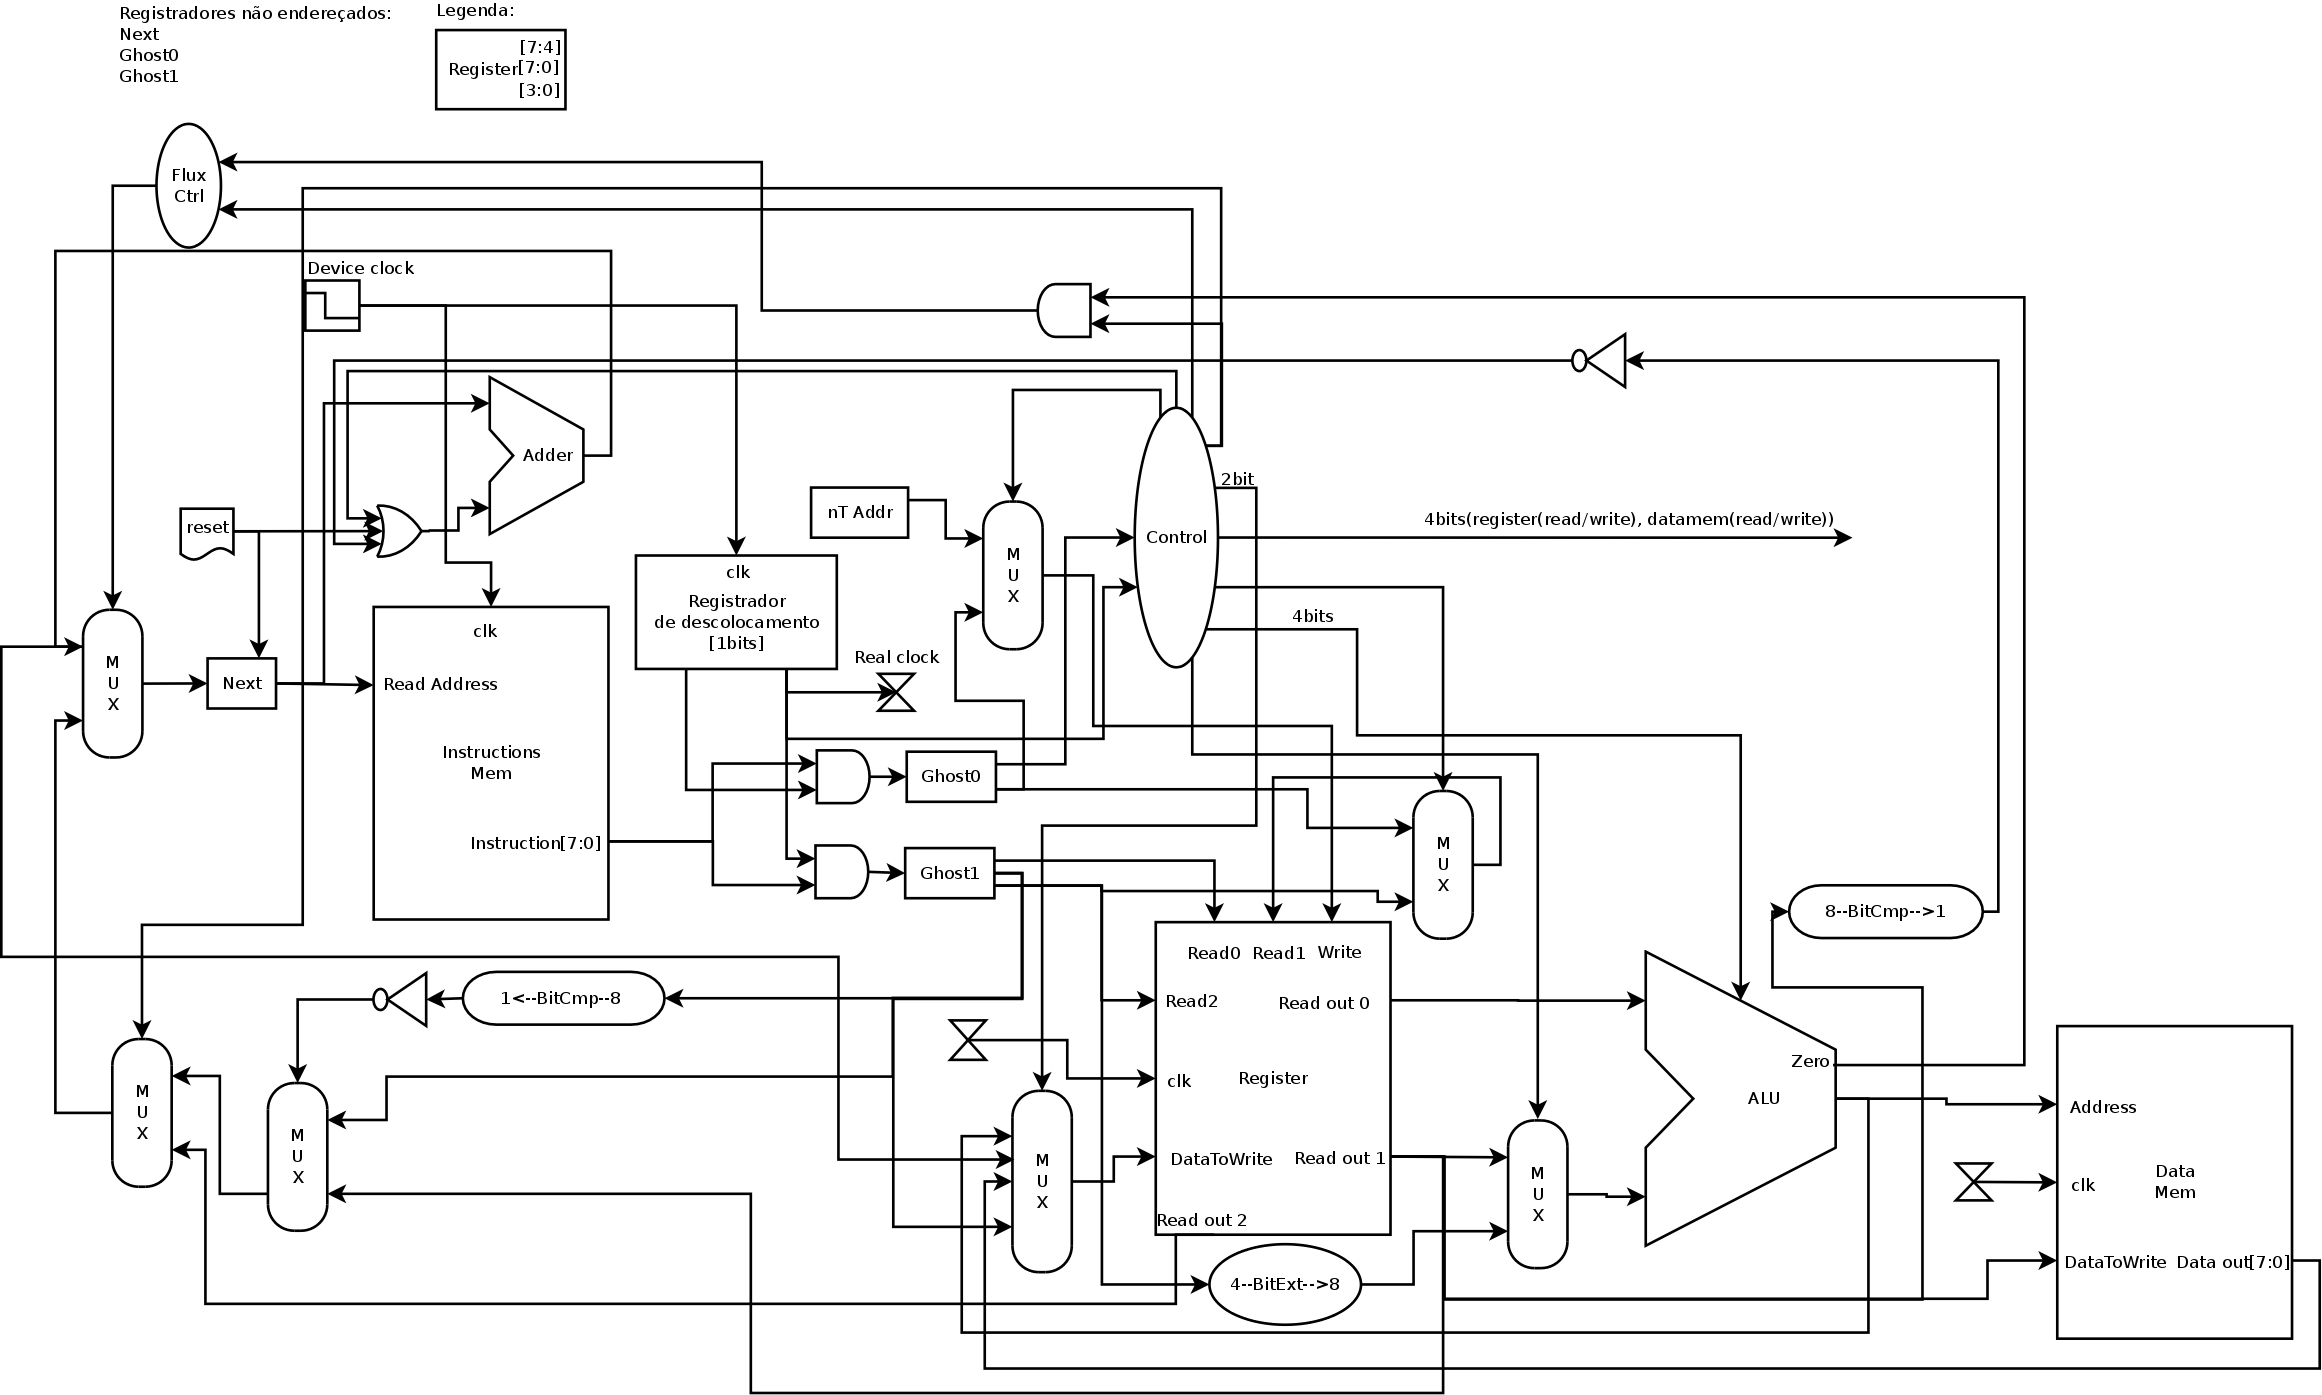
\includegraphics[scale=0.12]{nanoRiskDiagram.png}
	\caption{Caminho de dados nanoRisk}
	\label{Rotulo}
\end{figure}
Para a implementação do projeto de um processador de 8 bits com instruções que necessitam de 16 bits foi necessário adicionar dois registradores temporarios não endereçados para armazenar cada parte da instrução e dividir o clock por dois para as intruções usando um registrador de deslocamento de 1 bit(um bit sempre é um e outro sempre é zero), esse registrador de deslocamento também serve para alternar em qual registrador "ghost" será armazenado aquele pedaço de instrução. Os Bit Compacters(BitCmp) são uma porta lógica or para 8 entradas. Durante o desenvolvimento do diagrama, foi possivel observar algumas coisas desnecessárias que foram descritas no projeto, como por exemplo o registrador bp(base pointer) e a função la(load address) que poderia ser substituida pela função load constant sem problemas já que não há calculos de alinhamento.
\newpage
\subsection{Bits de controle}
Há 9 saídas do controle, que totalizam 16 bits de cotrole. As nove saídas são descritas abaixo seguindo a ordem de cima para baixo no diagrama do caminho de dados.
\begin{itemize}
	\item 1-Temporary Write(tmpwr)\\
	Bit para definir se o registrador de escrita vai ser o temporário se for zero ou o registrador passado na instrução se for um. Em uma nova versão do projeto seria possível alterar a estrutura da instruções para que as que usam o registrador temporário não precissasem passar ele como parâmetro. As funções de link que gravam o endereço de next+1, usam esse bit para gravar no registrador nT o valor de retorno, poderia ser usado o endereço de RA também mas não é o caso devido ao projeto.
	\item 2-Halt(hlt)\\
	Bit para definir o estado sleep, se ele for zero e o registrador de flag for diferente de zero o programa continua congelado nessa instrução. Um sinal externo de reset pode reiniciar o programa, ou caso haja uma modificação no projeto para adicionar outros cores um deles pode tirar desse estado também.
	\item 3-Jump(jmp)\\
	Define se a instrução é uma instrução de jump incondicional, se for um, o proximo endereço não virá de next+1
	\item 4-Branch(brc)\\
	Define se a instrução é uma instrução de branch condicional, se for um e a operação na ula retornar verdadeiro habilita o branch, o endereço virá da leitura 2 do banco de registradores. Esse campo de leitura é usado apenas para esse caso e caso mudasse o projeto inteiro das intruções seria possivel evita-lo passando o registrador de retorno primeiro, ou mudando a ordem apenas para esse tipo de instrução.
	\item 5-Register Write(rgw)\\
	Dois bits que definem o que vai ser escrito no registrador, o valor dos bits se encontra abaixo e após está seu significado, sendo que o primeiro é o mais significativo: 
	\subitem 00 - Resultado da ula.
	\subitem 01 - Próxima instrução.
	\subitem 10 - Valor lido na memória de dados.
	\subitem 11 - Constante passada pela instrução.
	\item 6-Input Output Control(ioc)\\
	Quatro bits que definem as entradas e saídas em termos de memória e registrador eles controlam escrita e leitura na memoria de dados e no banco de registradores. Sendo os bits 4,3,2 e 1 os bits desse sinal de controle do mais significativo pro menos significativo, eles repesentam:
	\subitem 4 - Habilita escrita no banco de registradores se for um.
	\subitem 3 - Habilita leitura no banco de registradores se for um.
	\subitem 2 - Habilita escrita na memória de dados se for um.
	\subitem 1 - Habilita leitura na memória de dados se for um.
	\item 7-Register Read(rgr)\\
	Bit que define de onde vem o segundo valor a ser lido no banco de registradores, se for zero será lido a partir do enderço passado nos ultimo quatro bits do primeiro byte da instrução, se for um será lido a partir do enderço passado nos ultimo quatro bits do segundo byte da instrução.
	\item 8-ALU Operation(alo)\\
	Quatro bits que definem qual operação será feita na ula. O códigos de cada operação estão abaixo e após está seu significado, lembrando q o primeiro bit é o mais significativo:
	\subitem 0000 - Adição, a saída é a soma das entradas.
	\subitem 0001 - Subtração do primeiro valor na ula pelo segundo, se o resultado for zero, define a saída zero como um.
	\subitem 0010 - Teste de flag, faz um \& lógico das entradas, se o resultado for verdadeiro para todos os bits onde a segunda entrada é um ele define a saída zero como um e o resultado será a subtração do primeiro pelo segundo, caso contrario a saída zero será zero e a saída sera a primeira entrada.
	\subitem 0011 - And, a saída é a operação lógica and das entradas.
	\subitem 0100 - Or, a saída é a operação lógica or das entradas.
	\subitem 0101 - Nor, a saída é a operação lógica nor das entradas.
	\subitem 0110 - Less, faz a subtração da segunda entrada pela primera, define a saída zero como um se o valor for negativo.
	\subitem 0111 - Shift left, a saída é a primeira entrada deslocada para a esquerda o n vezes, onde n é o valor da segunda entrada
	\subitem 1000 - Shift right, a saída é a primeira entrada deslocada para a direita o n vezes, onde n é o valor da segunda entrada
	\subitem 1001 - Não usado
	\subitem 1010 - Não usado
	\subitem 1011 - Não usado
	\subitem 1100 - Não usado
	\subitem 1101 - Não usado
	\subitem 1110 - Não usado
	\subitem 1111 - Não usado
	\item 9-ALU Argument(ala)\\
	Bit que define segundo argumento da ula, pode ser um valor lido no banco de registradores se for zero ou uma constante/endreço passada pela função se for um.
\end{itemize}
\subsection{Valores de controle especificos}
A tabela abaixo contém os sinais de controle para cada função do processaodor nanoRisk, após analizar atentamente a tabela é possivel ver que podem ser feitas vária modificações para simplificar e diminuir a quantidade de bits de controle mas deixando tudo menos didatico.
\begin{table}[H]
	\centering
	\caption{Controle de instruções}
	\label{tab:Controle de instruções}
	\begin{tabular}{c c c c c c c c c c}
		\hline
		Instrução & tmpwr & hlt & jmp & brc & rgw & ioc & rgr & alo & ala \\
		\hline
		slp & X & 0 & 0 & 0 & XX & 0100 & 0 & XXXX & X \\
		brq & X & 1 & 0 & 1 & XX & 0100 & 0 & 0001 & 0 \\
		brf & 1 & 1 & 0 & 1 & 00 & 1100 & 0 & 0010 & 0 \\
		add & 1 & 1 & 0 & 0 & 00 & 1100 & 1 & 0000 & 0 \\
		sub & 1 & 1 & 0 & 0 & 00 & 1100 & 1 & 0001 & 0 \\
		and & 1 & 1 & 0 & 0 & 00 & 1100 & 1 & 0011 & 0 \\
		or & 1 & 1 & 0 & 0 & 00 & 1100 & 1 & 0100 & 0 \\
		nor & 1 & 1 & 0 & 0 & 00 & 1100 & 1 & 0101 & 0 \\
		slt & 1 & 1 & 0 & 0 & 00 & 1100 & 1 & 0110 & 0 \\
		sr & 1 & 1 & 0 & 0 & 00 & 1100 & 1 & 1000 & 0 \\
		sl & 1 & 1 & 0 & 0 & 00 & 1100 & 1 & 0111 & 0 \\
		jr & 0 & 1 & 1 & 0 & 01 & 1100 & 0 & XXXX & X \\
		la & 1 & 1 & 0 & 0 & 11 & 1000 & X & XXXX & X \\
		lc & 1 & 1 & 0 & 0 & 11 & 1000 & X & XXXX & X \\
		lw & 1 & 1 & 0 & 0 & 10 & 1101 & 0 & 0000 & 1 \\
		sw & X & 1 & 0 & 0 & XX & 0110 & 0 & 0000 & 1 \\
		\hline
	\end{tabular}
\end{table}
\newpage
\section{Caminho das instruções}
O caminho de dados especificos das instruções de acordo com o tipo pode ser visto nas imagens abaixo.
\begin{figure}[H]
	\centering
	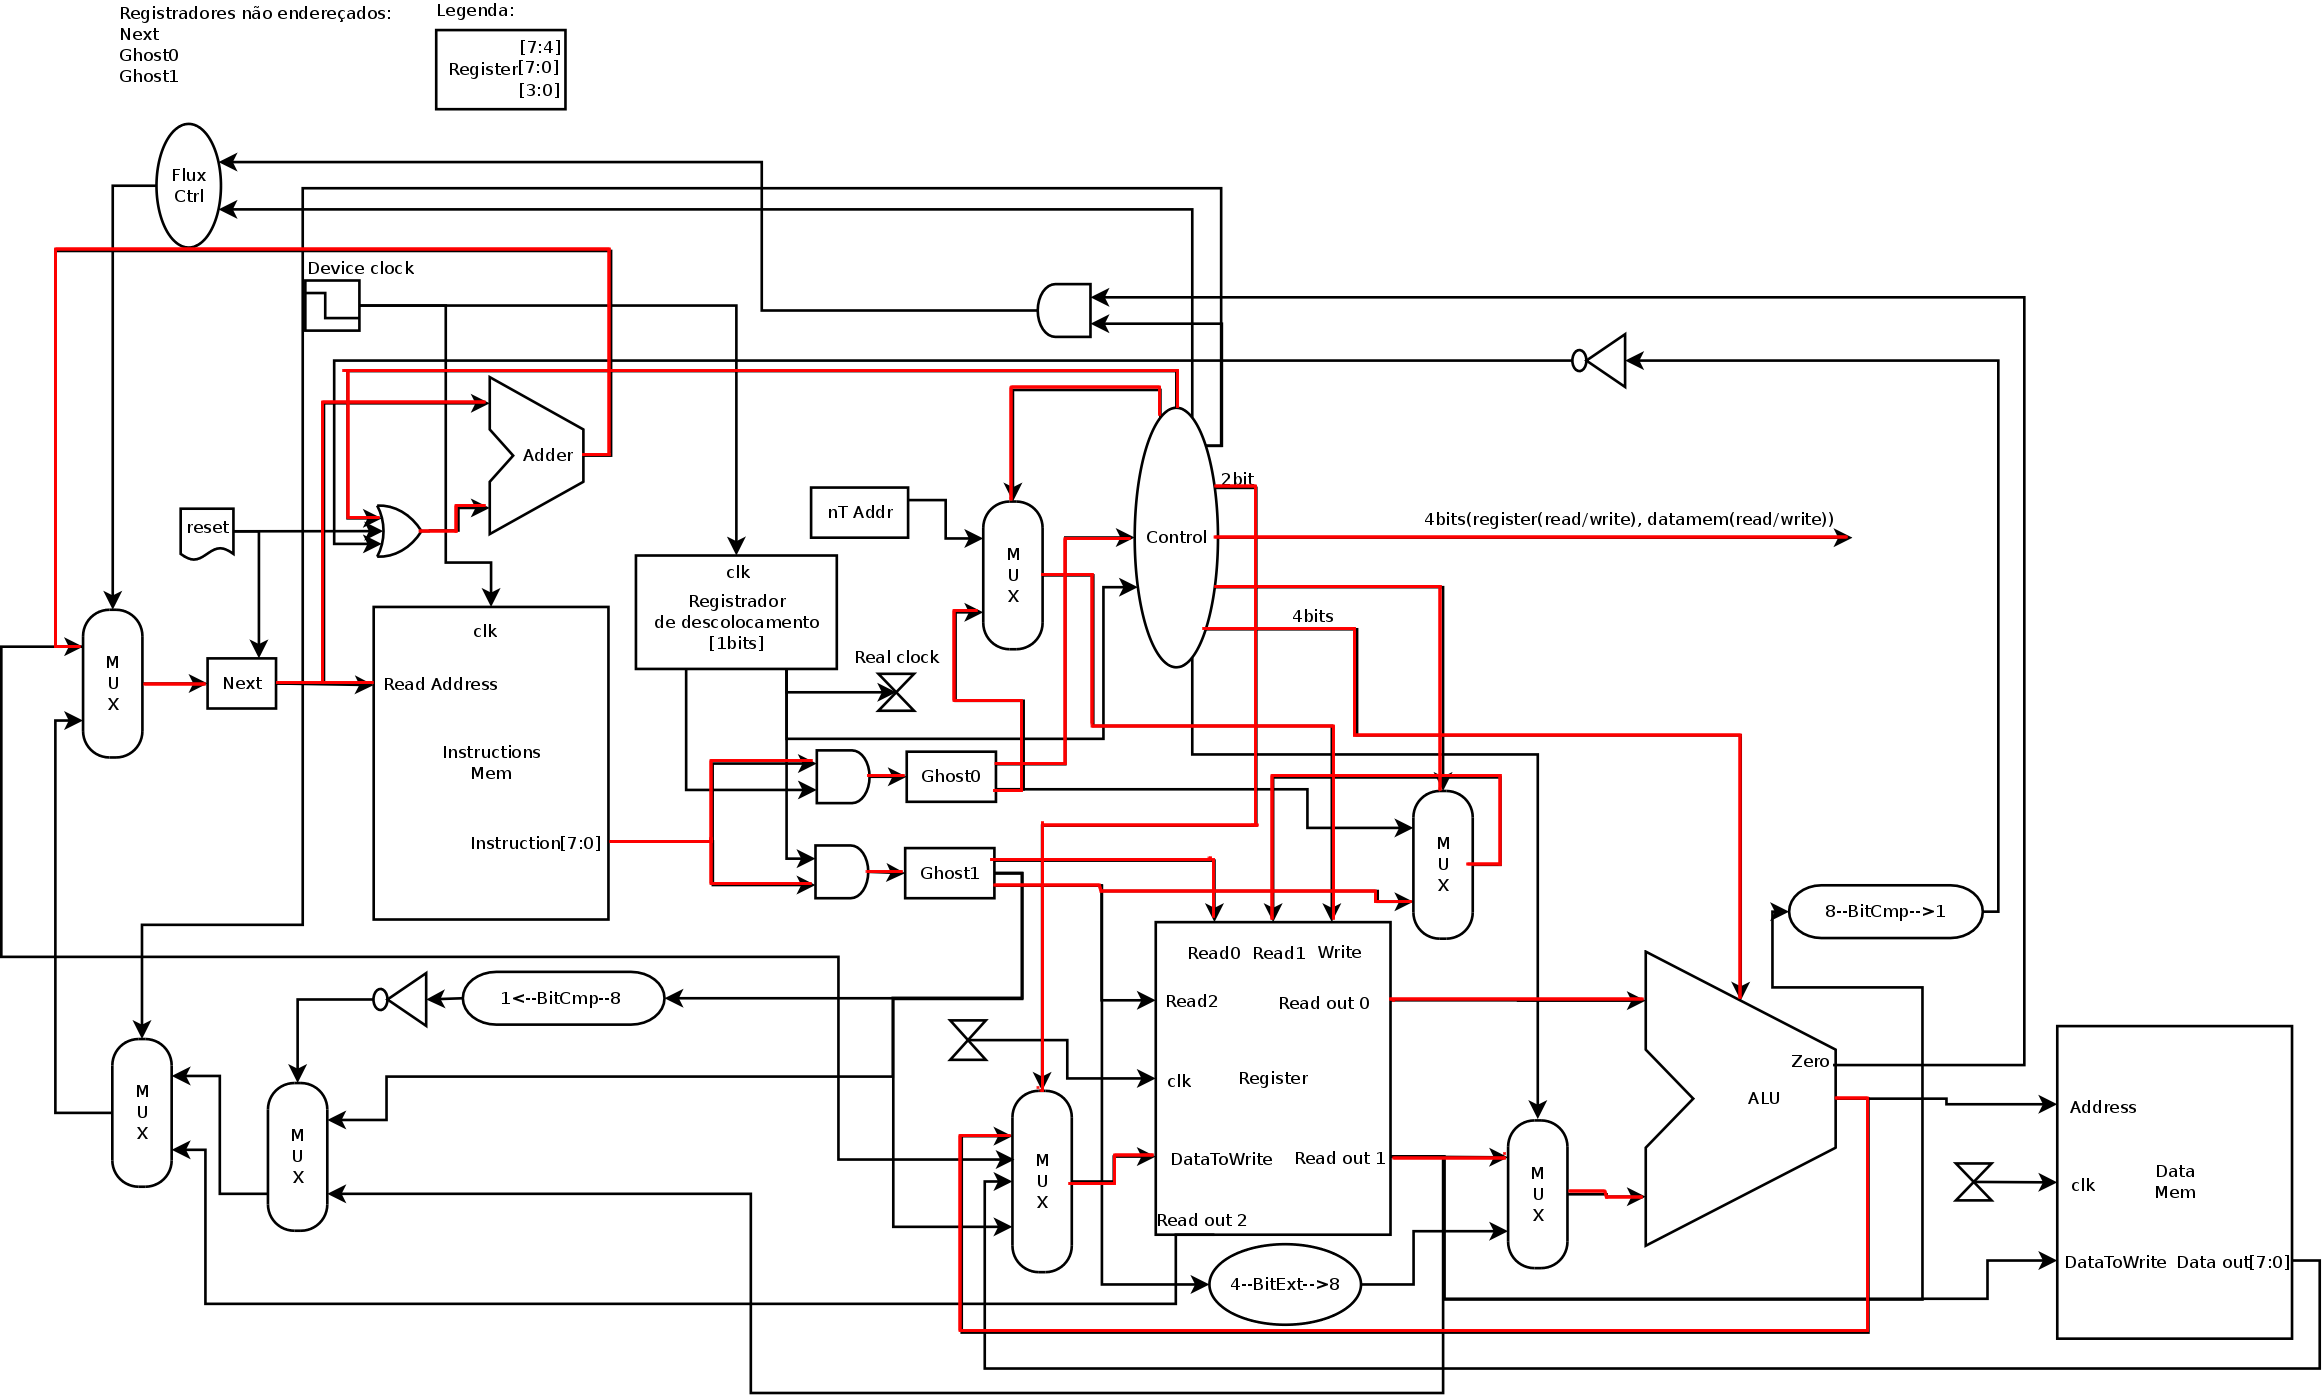
\includegraphics[scale=0.12]{dp_3r.png}
	\caption{Caminho de dados instruções lógicas e aritméticas}
	\label{Rotulo}
\end{figure}
\begin{figure}[H]
	\centering
	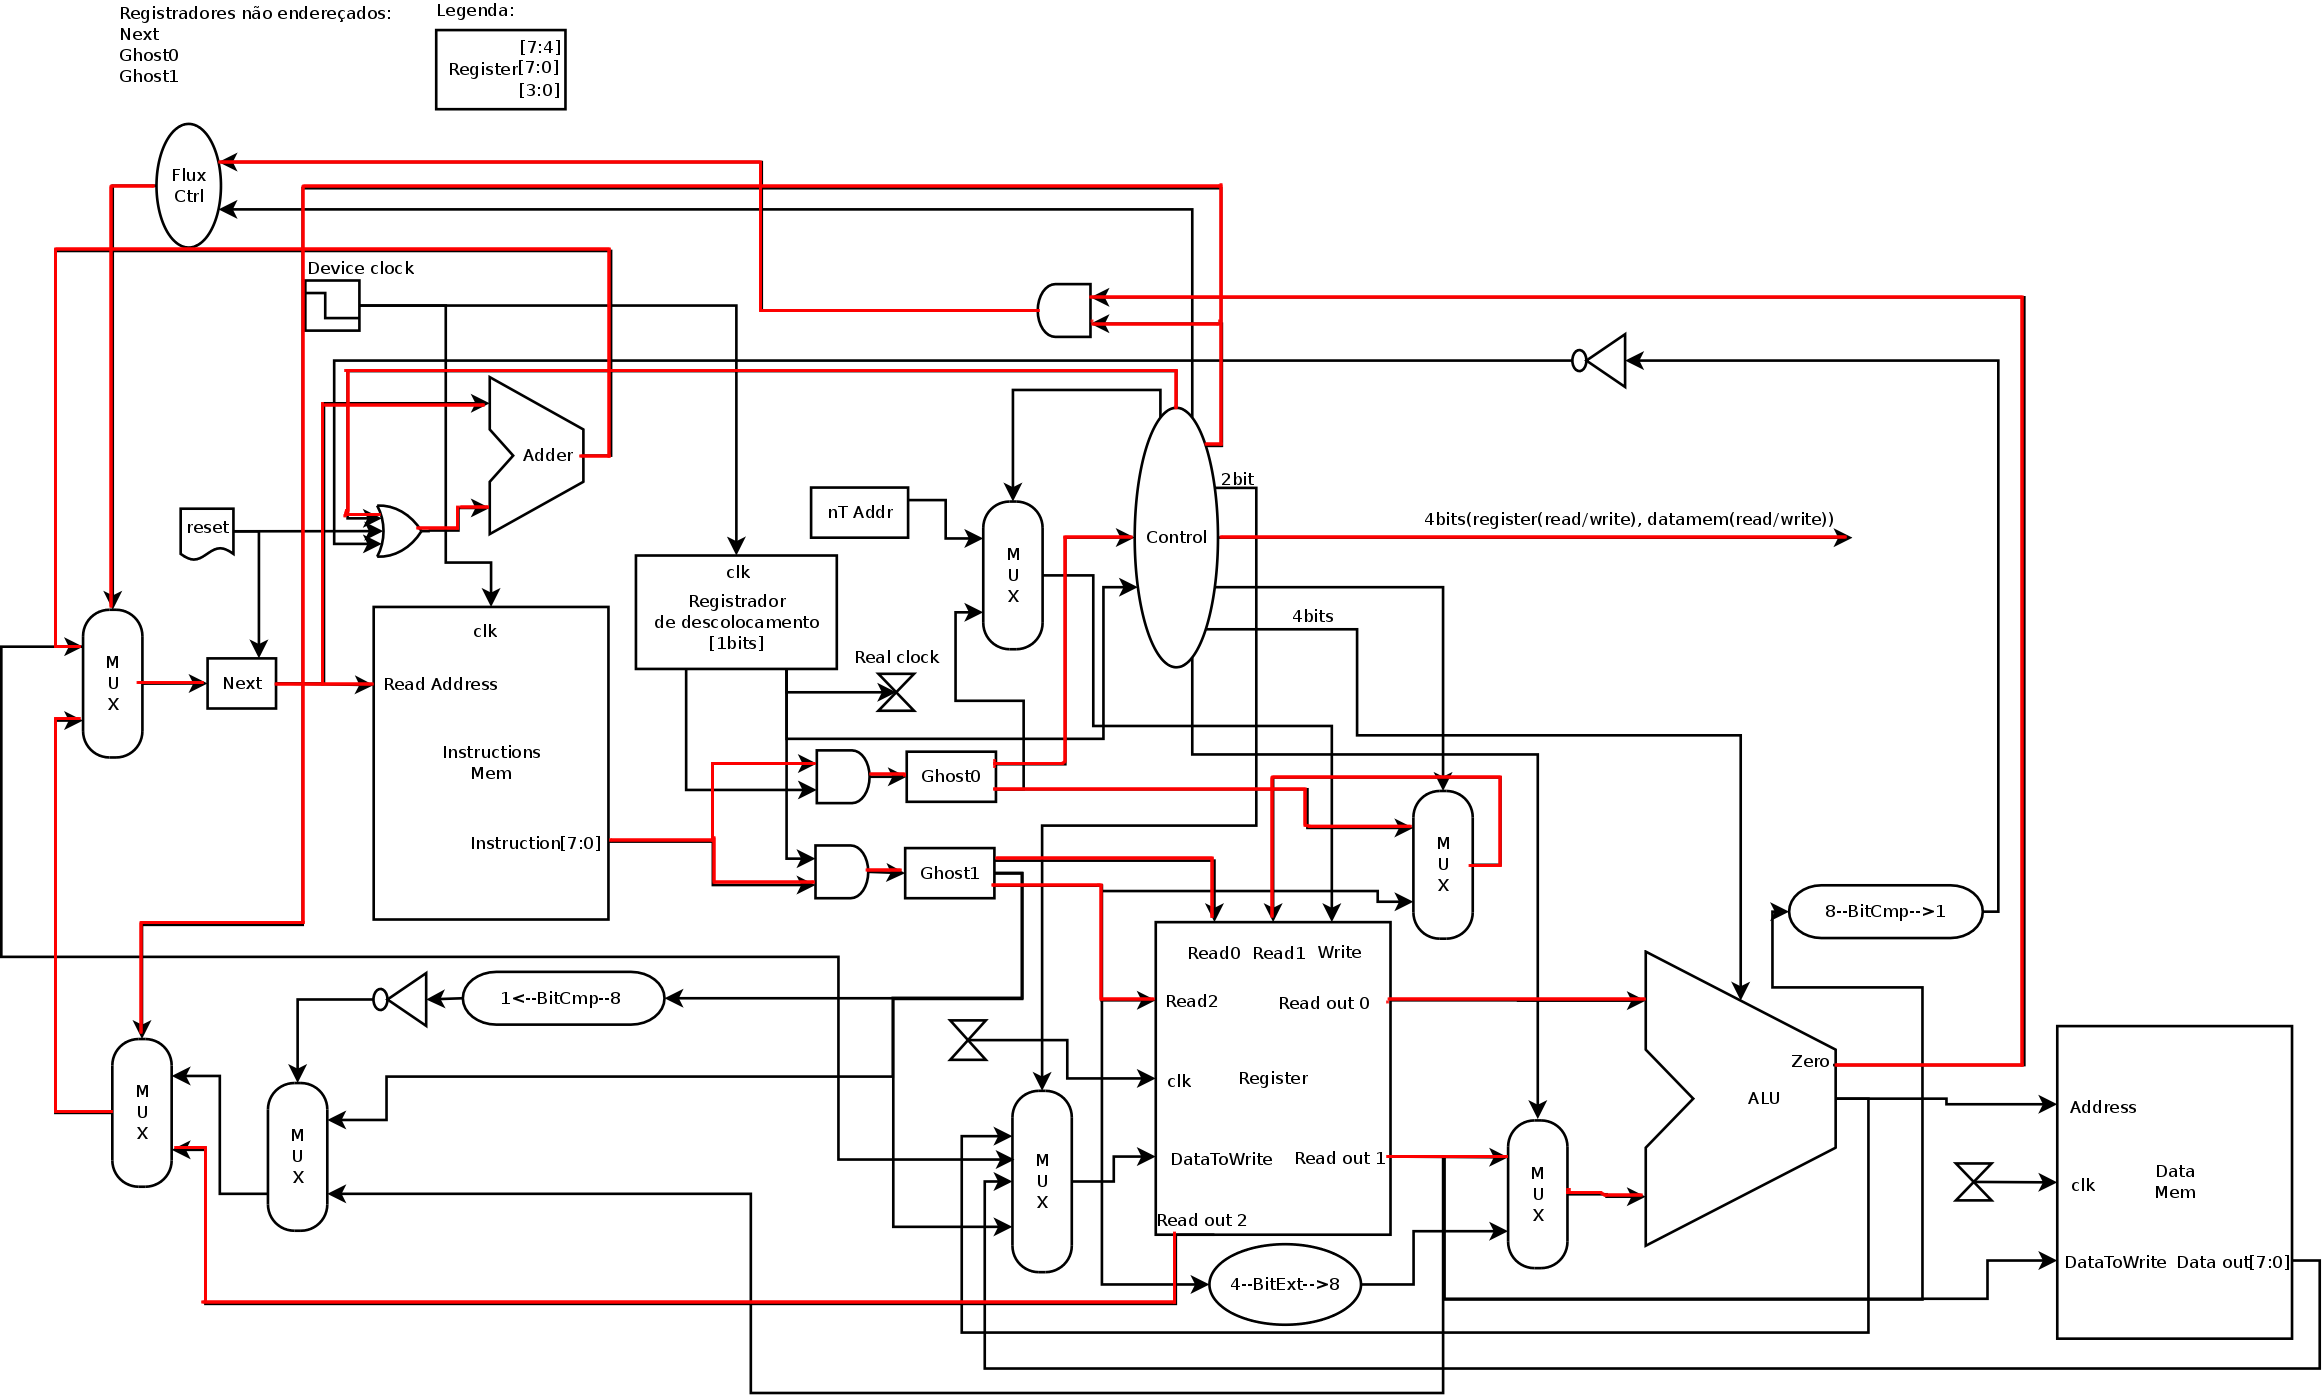
\includegraphics[scale=0.12]{dp_branch.png}
	\caption{Caminho de dados instruções de branch}
	\label{Rotulo}
\end{figure}
\begin{figure}[H]
	\centering
	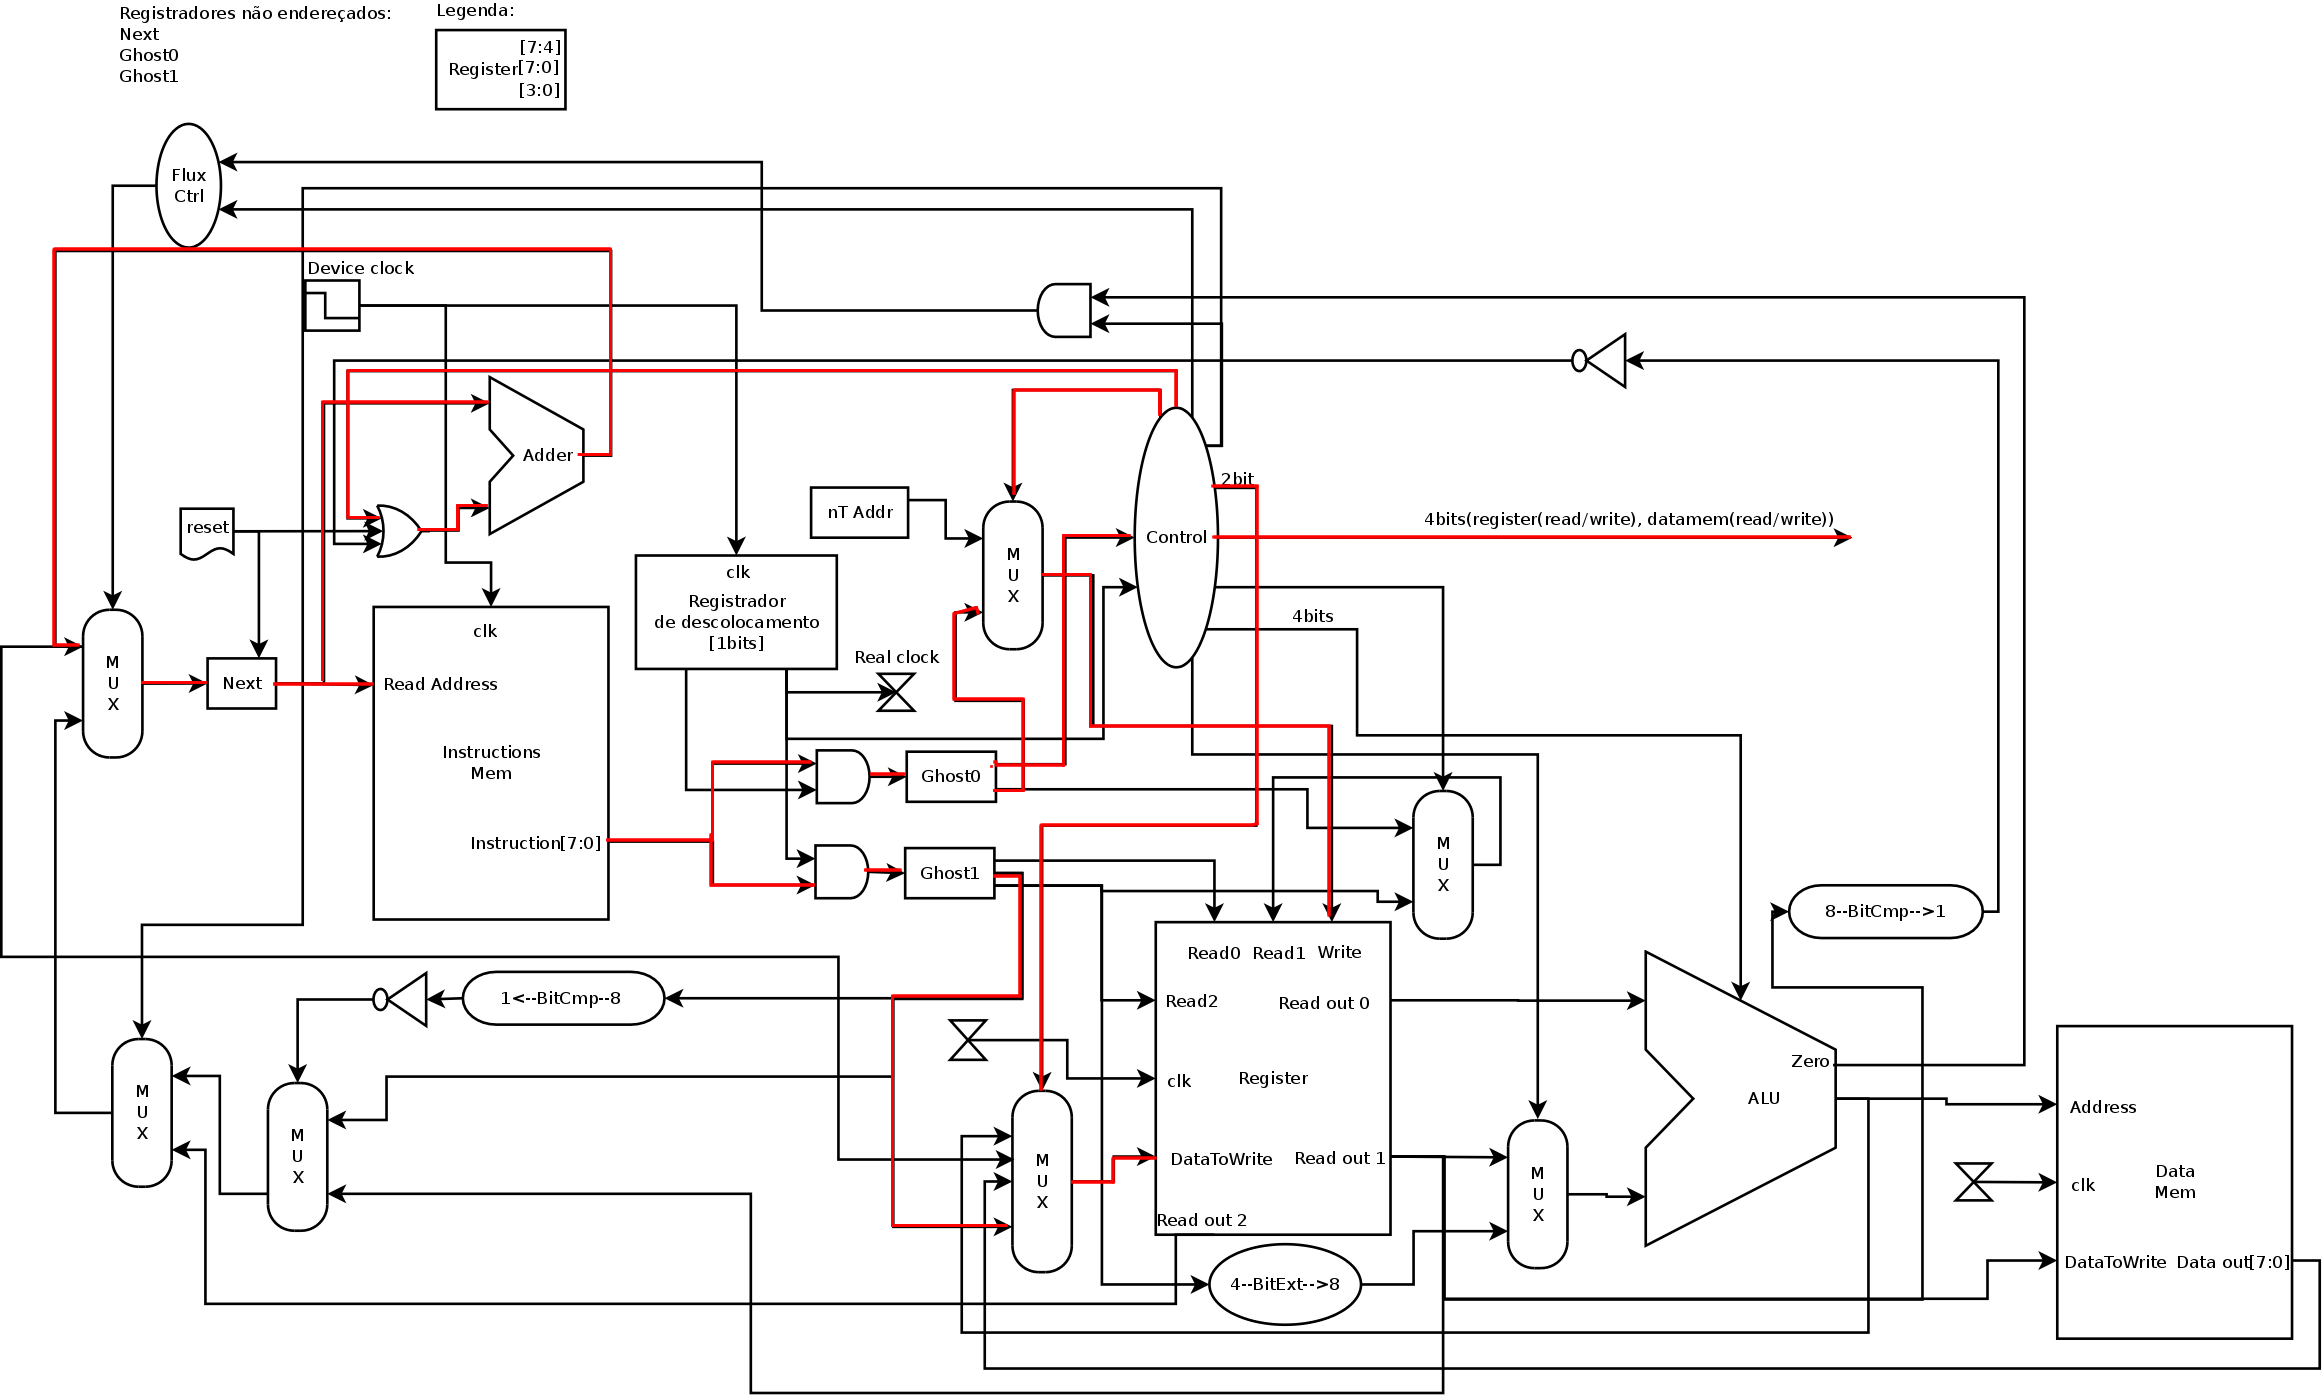
\includegraphics[scale=0.12]{dp_k.png}
	\caption{Caminho de dados intruções load address/constant}
	\label{Rotulo}
\end{figure}
\begin{figure}[H]
	\centering
	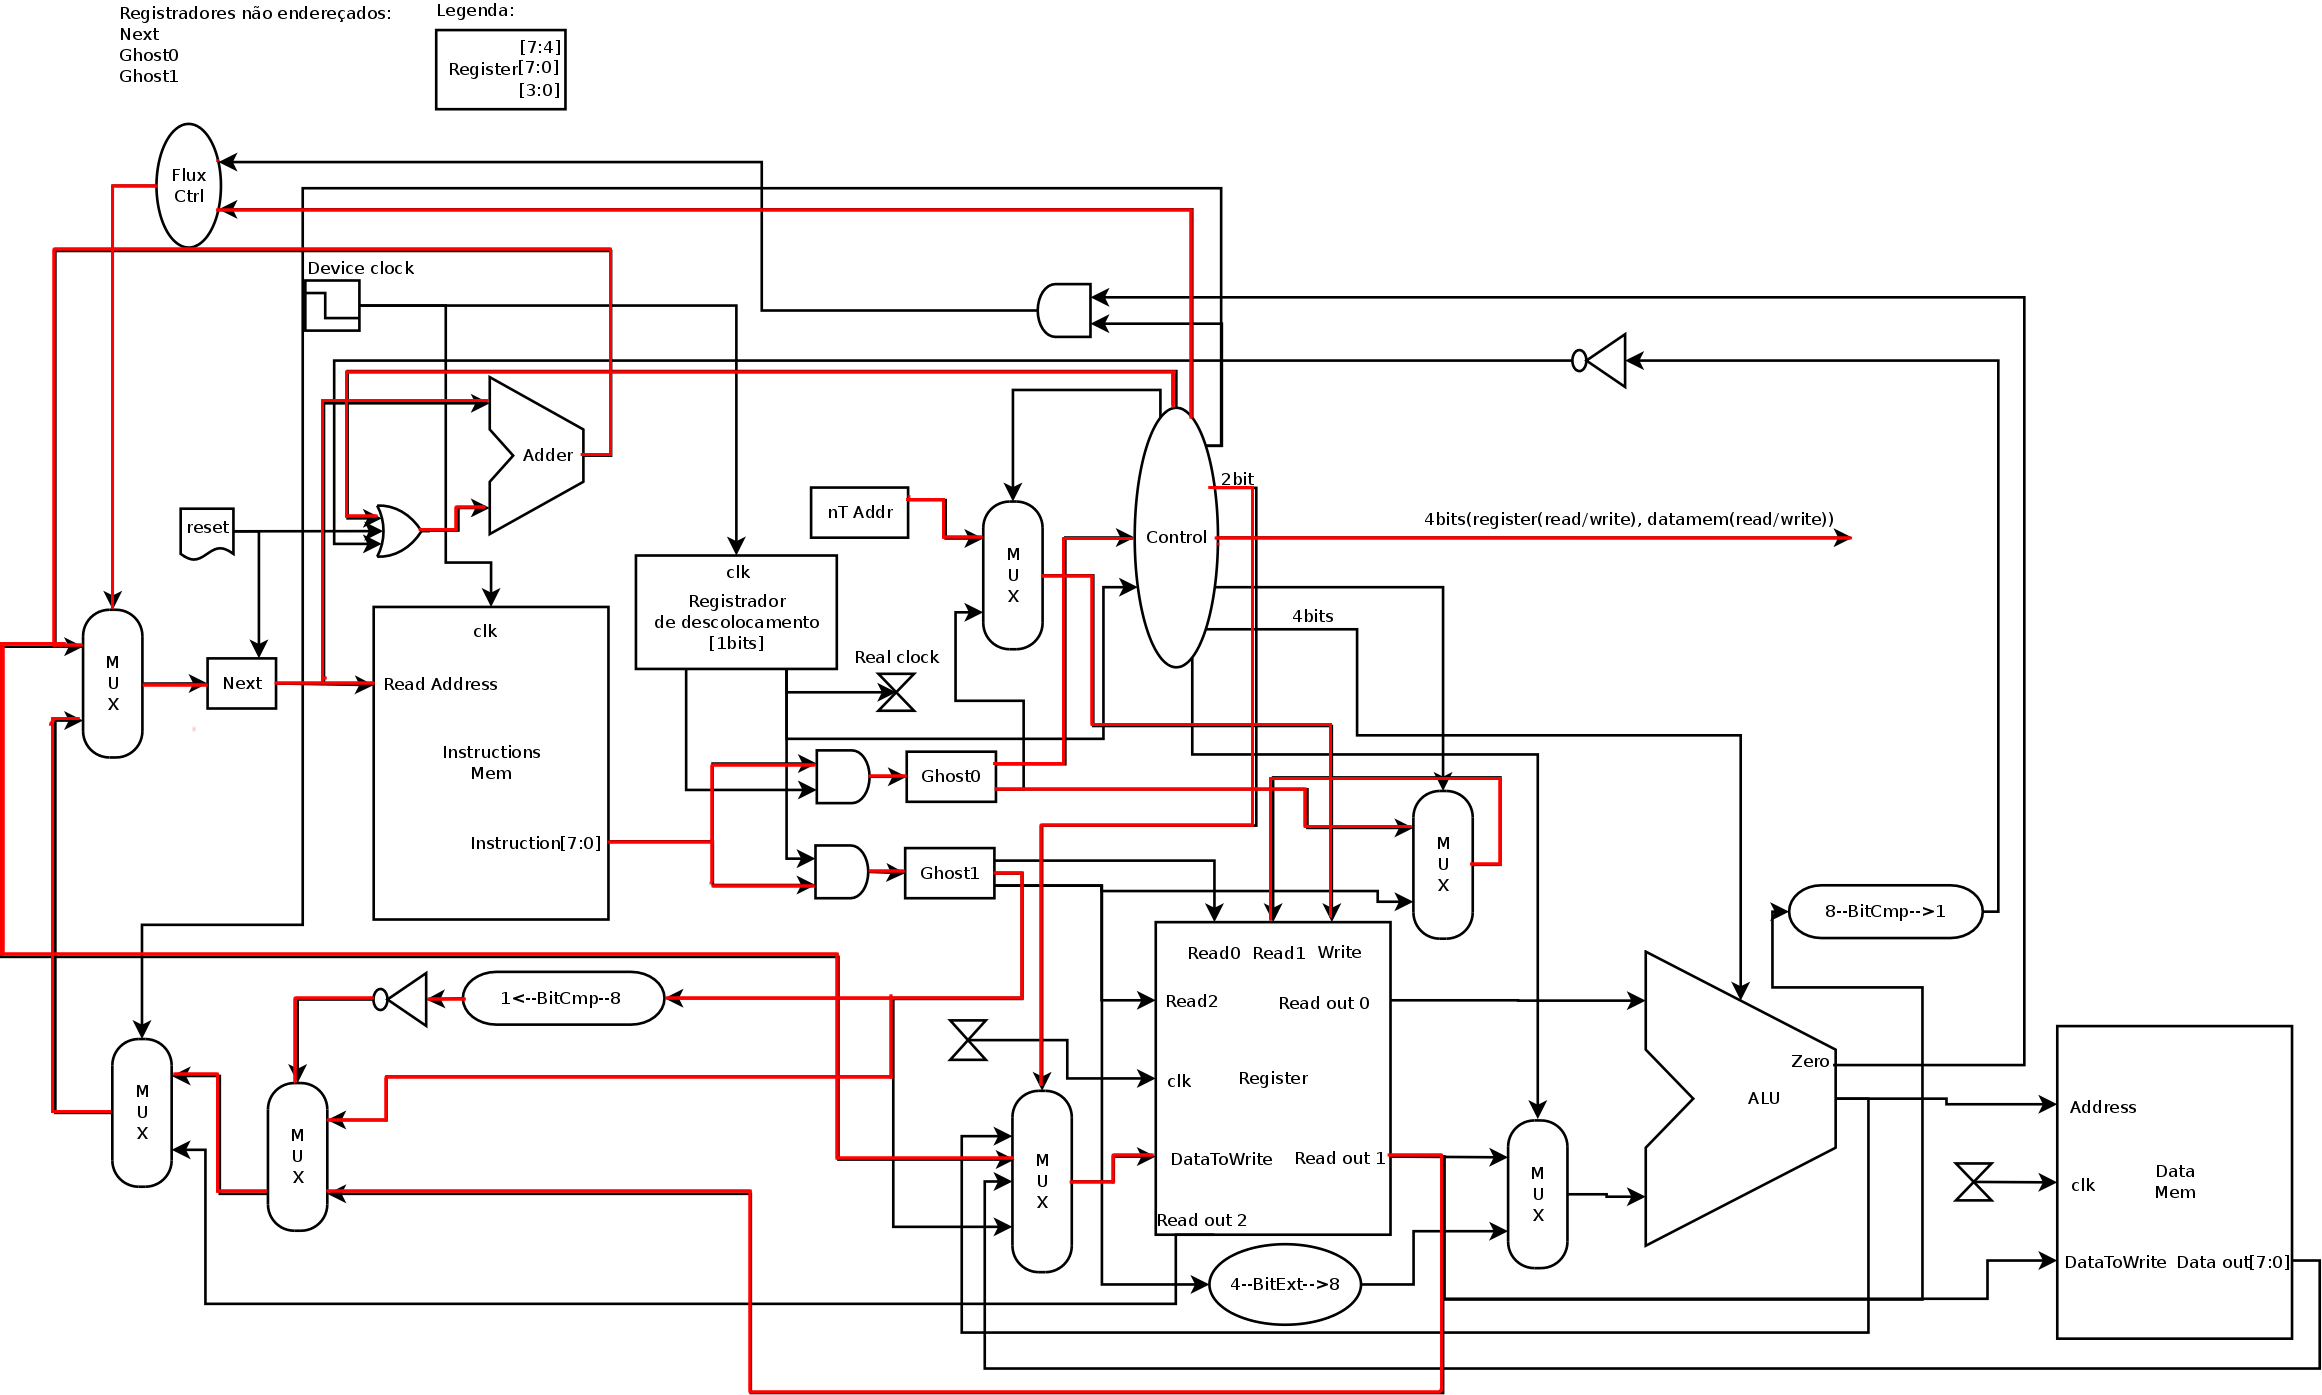
\includegraphics[scale=0.12]{dp_jump.png}
	\caption{Caminho de dados instruções de jump}
	\label{Rotulo}
\end{figure}
\begin{figure}[H]
	\centering
	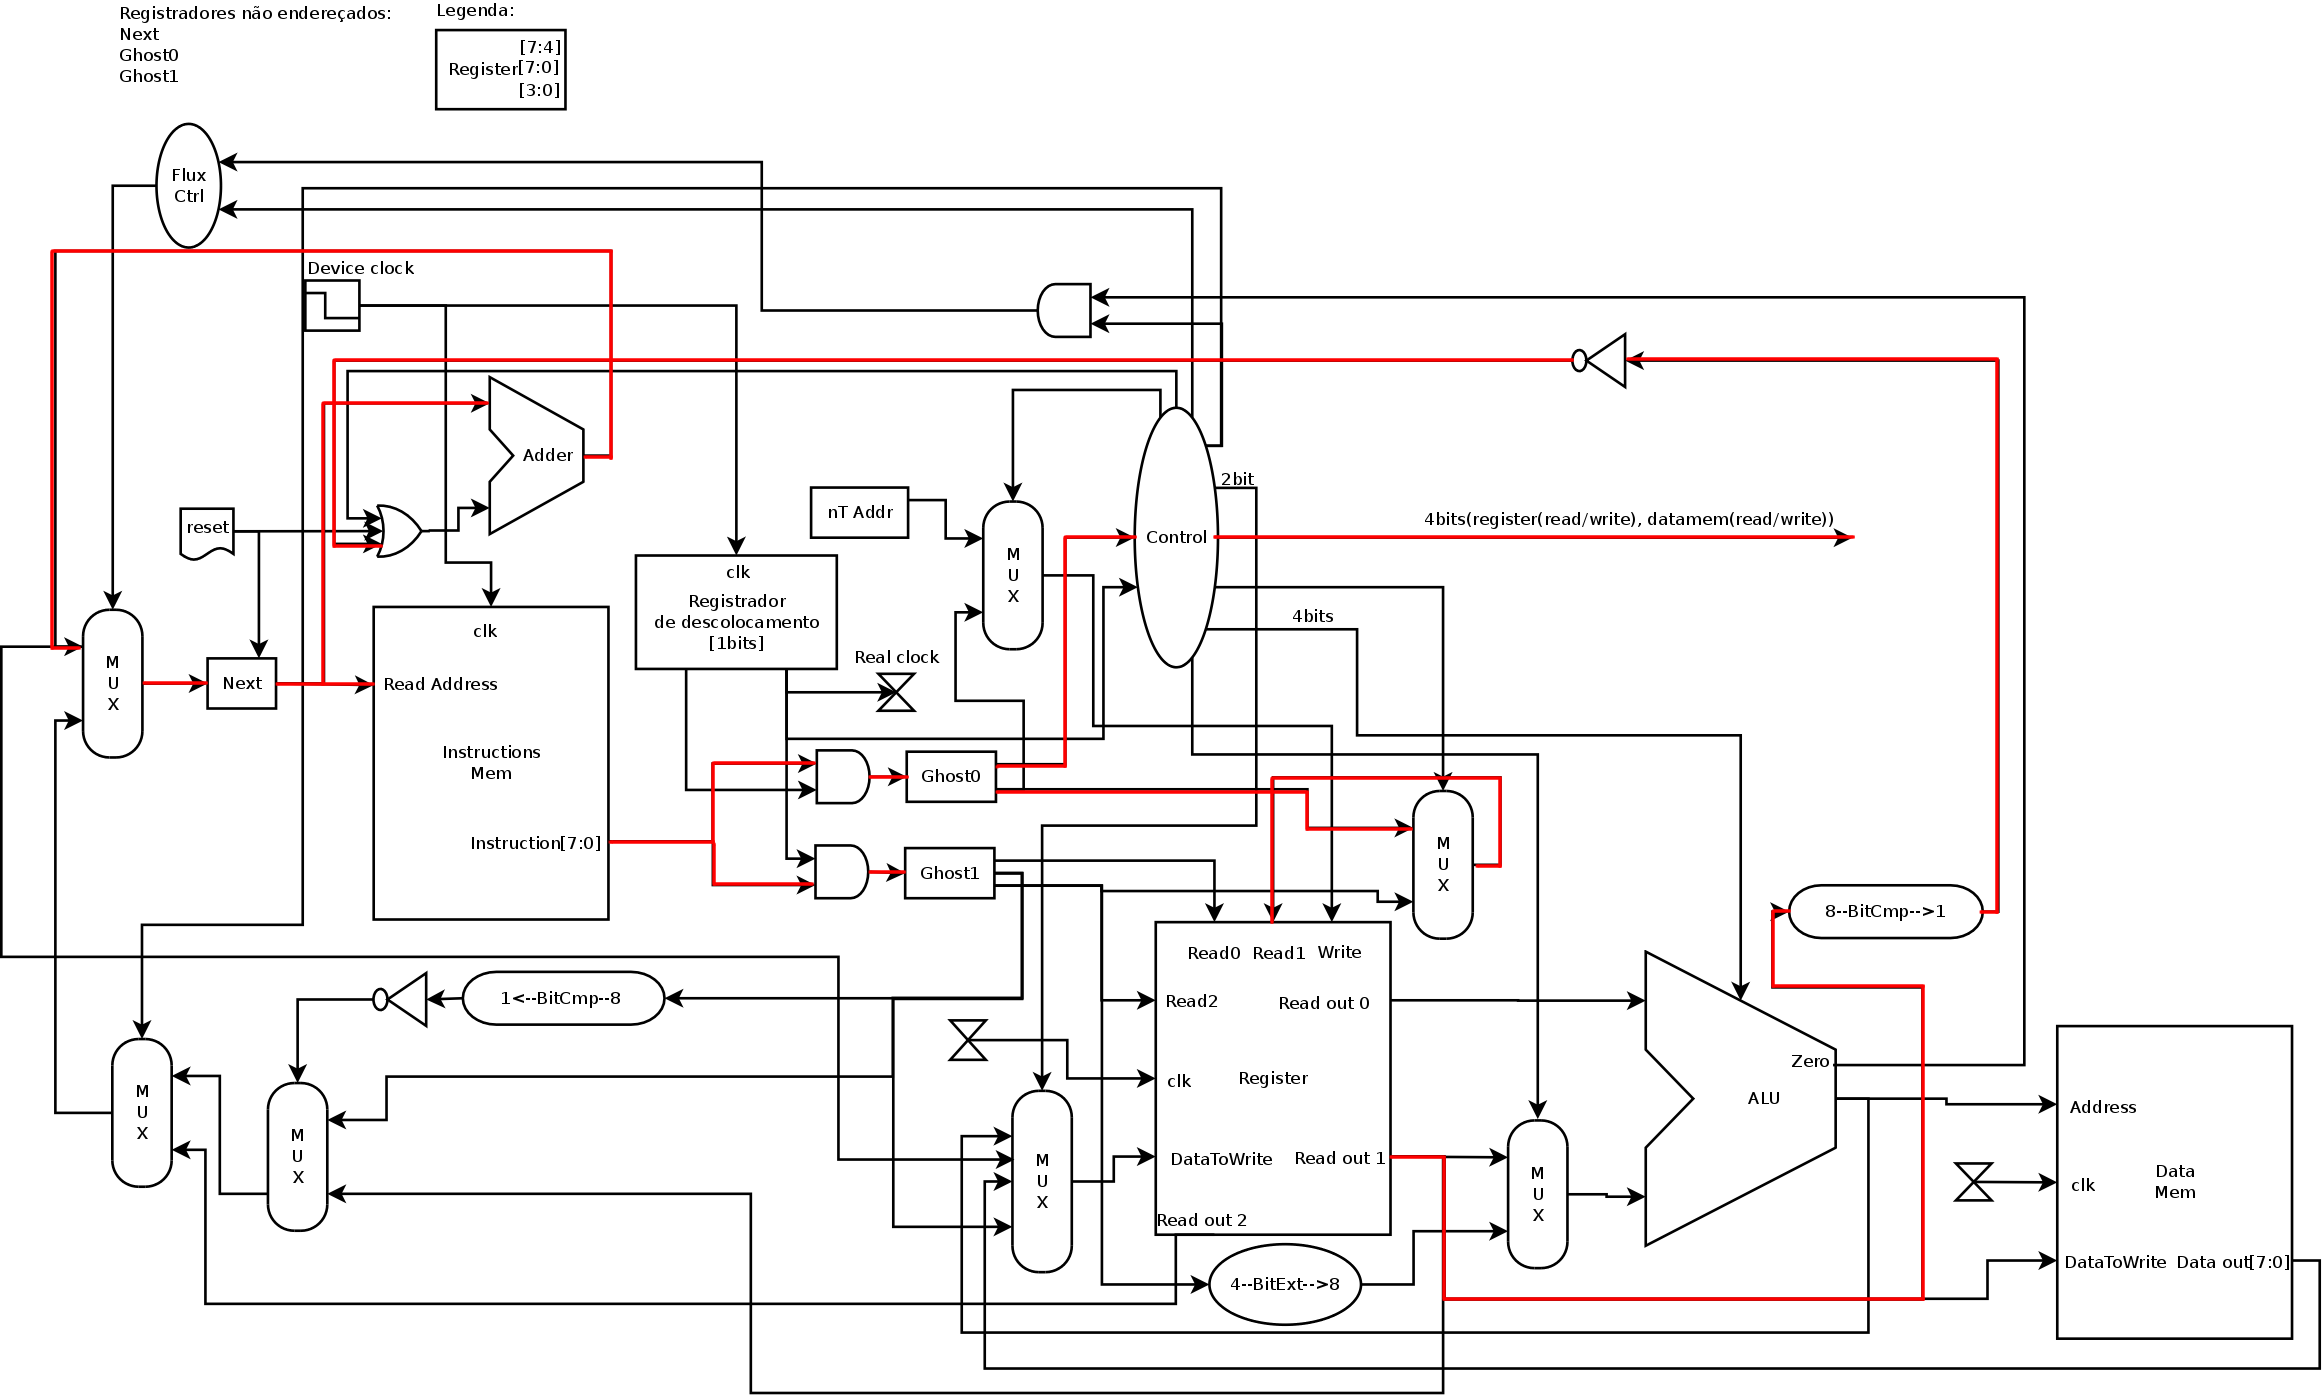
\includegraphics[scale=0.12]{dp_sleep.png}
	\caption{Caminho de dados intrução sleep}
	\label{Rotulo}
\end{figure}
\begin{figure}[H]
	\centering
	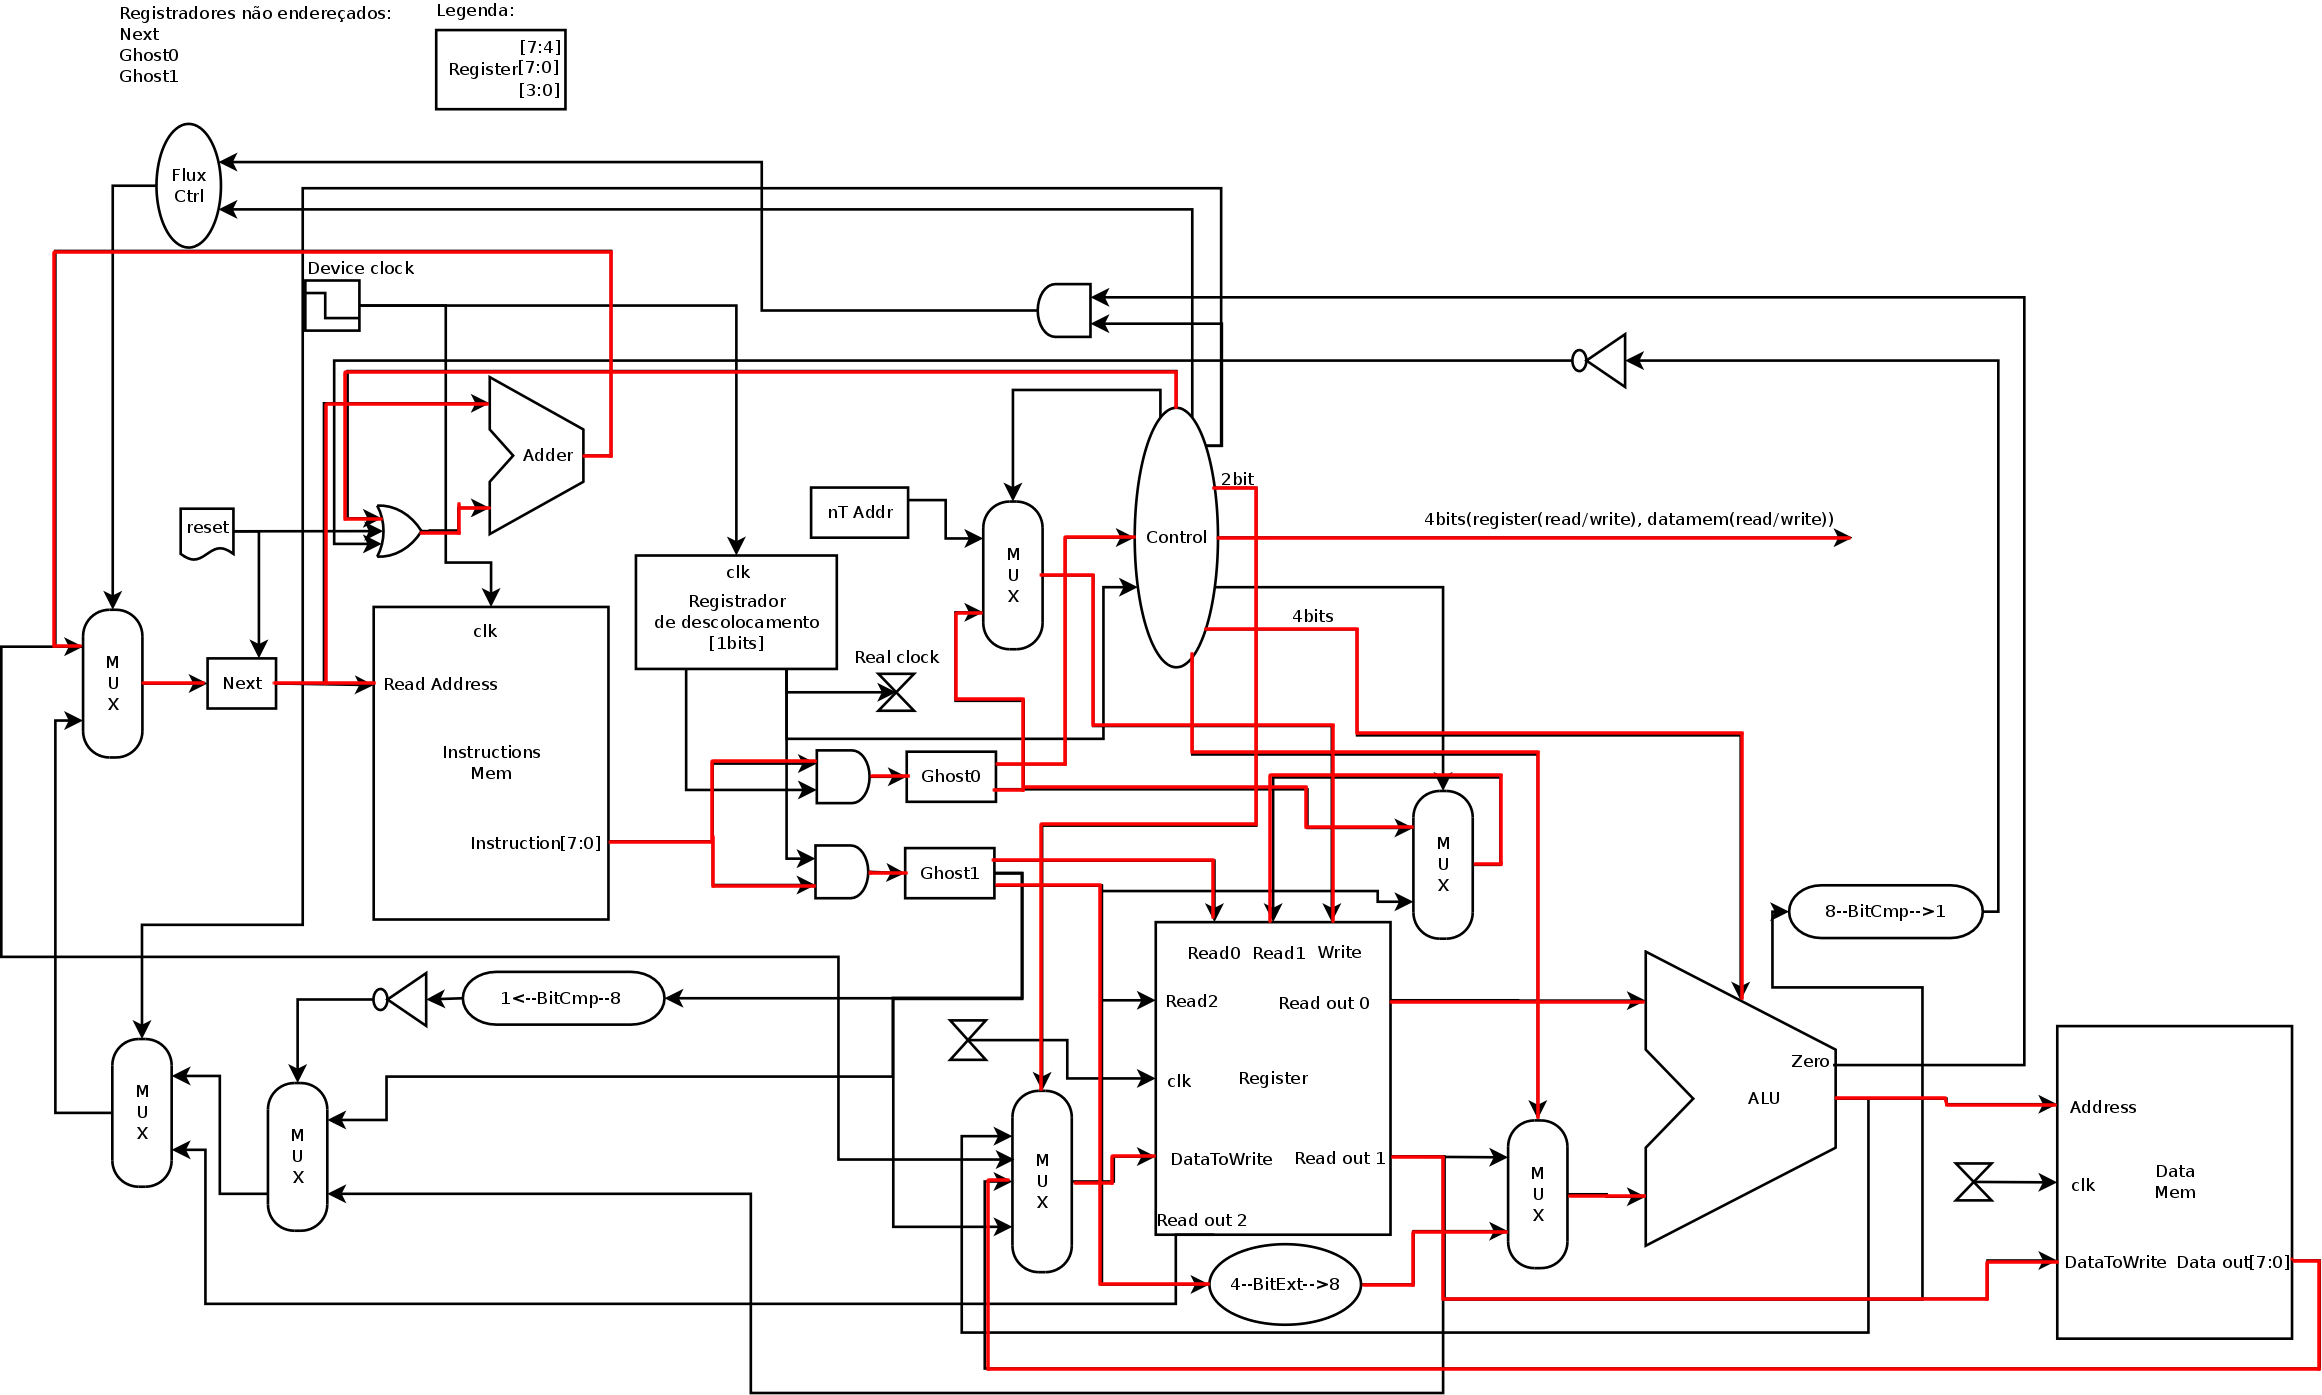
\includegraphics[scale=0.12]{dp_mem.png}
	\caption{Caminho de dados intruções sw/lw}
	\label{Rotulo}
\end{figure}
\newpage
\section{Alterações no projeto}
\subsection{Overflow}
Durante a relização da prática foi notado que não havia sido projetado uma forma de gravar as exceções de overflow, então foi adicionado no banco de registradores a entrada "ovrflw", que sai da ALU, essa entrada de dois bits informa estados de overflow que são gravados de forma assincrona no registrador flg, o bit mais significativo é o underflow e o menos significativo é o overflow. O overflow é gravado usando o ou lógico, assim conserva os dados gravados previamente.
\subsection{Sincronização}
Um caso de erro que pode ocorrer devido alguma falha eletrica, lógica ou humana é o estado onde o endereço de next é um numero impar e o registrador ghost atual é o 0, isso faria com que o programa não funcionasse, então uma forma de forçar para que isso não ocorra de forma alguma é adicionar uma porta logica AND, na saída 1 do registrador de deslocamento(real clock) e a outra entrada dessa AND seria o bit menos significativo de next, assim impediariamos o clock de funcionar na hora errada. Seria necessário também colocar uma AND na entrada de clock de ghost0 juntamente com o bit menos significativo de next invertido, para evitar a gravação em um momento errado.
\section{Componentes de memória}
Foram implementados em verilog registrador, registrador de deslocamento, banco de registradores e memória, abaixo podemos ver o código verilog desses componentes, acima do código de cada há um comentario explicando suas entradas e saídas.
\lstinputlisting[language={v}]{MemoryComponents/MemoryComponents.v}
\subsection{Simulação}
Para verificar o funcionamento dos componentes foi criado um código extra para simulações que é o código abaixo:
\lstinputlisting[language={v}]{MemoryComponents/MemoryComponents_Test.v}
\subsubsection{Resultados}
As imagens abaixo são prints das simulações e serão usadas para analisar o funcionamento do código.
\begin{itemize}
	\item Registrador de Deslocamento\\
	\begin{figure}[H]
		\centering
		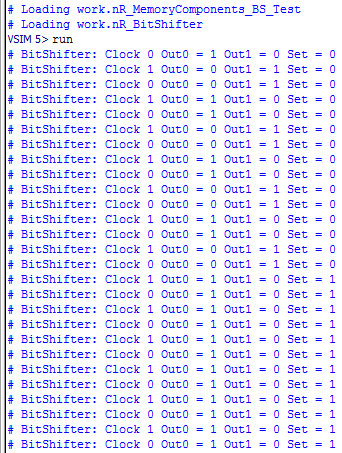
\includegraphics[scale=0.7]{BSsimu.PNG}
		\caption{Simulação do registrador de deslocamento}
		\label{Rotulo}
	\end{figure}
	Podemos ver que quando o clock altera seu estado de zero para um, o circuito faz o deslocamento dos bits e de forma assincrona, quando set tem nivel logico alto o registrador vai para o estado inicial, logo o circuito funciona corretamente.
	\item Registrador\\
	\begin{figure}[H]
		\centering
		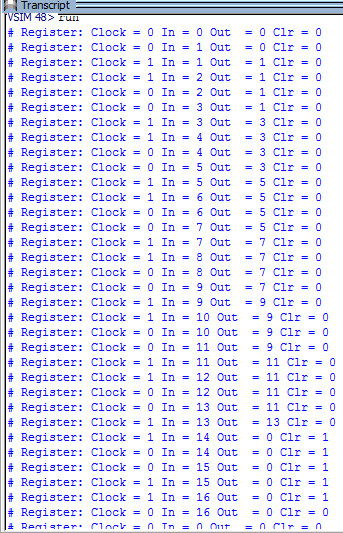
\includegraphics[scale=0.7]{REGsimu0.PNG}
		\caption{Simulação do registrador de deslocamento}
		\label{Rotulo}
	\end{figure}
	\begin{figure}[H]
		\centering
		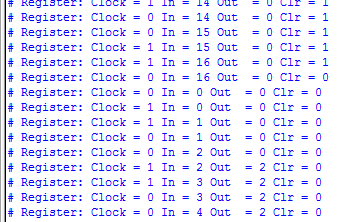
\includegraphics[scale=0.7]{REGsimu1.PNG}
		\caption{Simulação do registrador de deslocamento}
		\label{Rotulo}
	\end{figure}
	\vfill
	Quando o clock tem borda de subida, o valor na entrada é gravado, quando temos borda de subida o valor é lido corretamente. Podemos ver tambem que o controle de leitura e escrita tambem funciona, permitindo ou nao leitura e escrita. O sinal assincrono de clear também está funcionado, zerando os valores quando tem nivel logico alto.
	\item Banco de Registradores\\
	\begin{figure}[H]
		\centering
		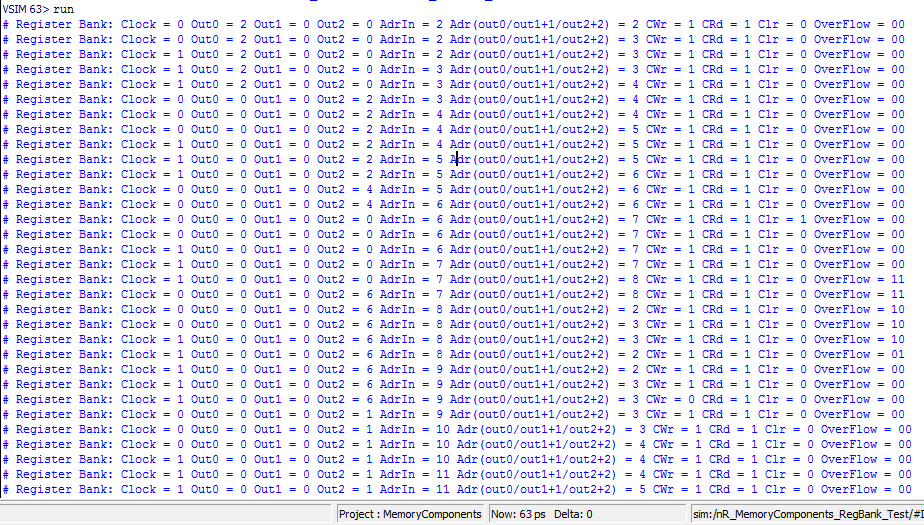
\includegraphics[scale=0.6]{BANKsimu.PNG}
		\caption{Simulação do banco de registradores, valor inicial zero}
		\label{Rotulo}
	\end{figure}
	Quando o clock tem borda de subida, o valor no endereco de entradada(que é o mesmo da entrada nesse caso) é gravado, quando temos borda de subida o valor é lido corretamente. Podemos ver tambem que o controle de leitura e escrita tambem funciona, permitindo ou nao leitura e escrita. O sinal assincrono de clear também está funcionado, zerando os valores quando tem nivel logico alto.
	\begin{figure}[H]
		\centering
		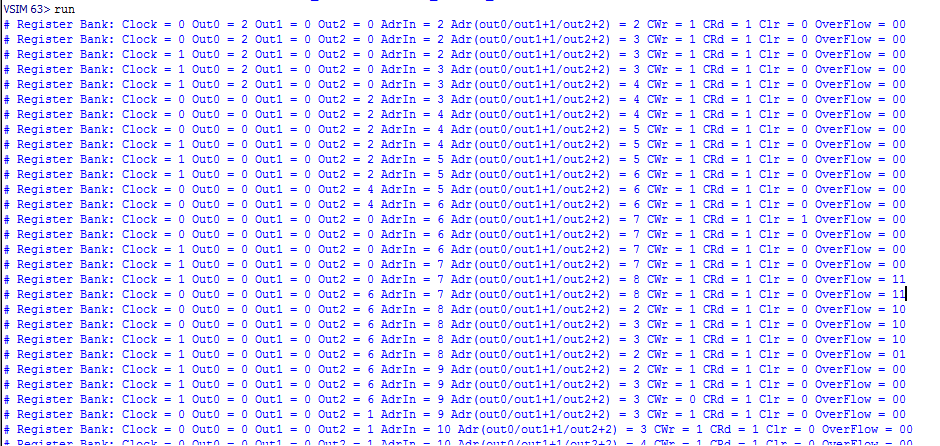
\includegraphics[scale=0.6]{BANKsimu-startedvalues.PNG}
		\caption{Simulação do banco de registradores, valor inicial igual à posição}
		\label{Rotulo}
	\end{figure}
	Nesse caso o banco de registradores ja estava inicializado, o valor de cada posição era o indice da mesma, isso é perciptivel antes da primeira vez que clear é '1'.
	\vfill
	\begin{figure}[H]
		\centering
		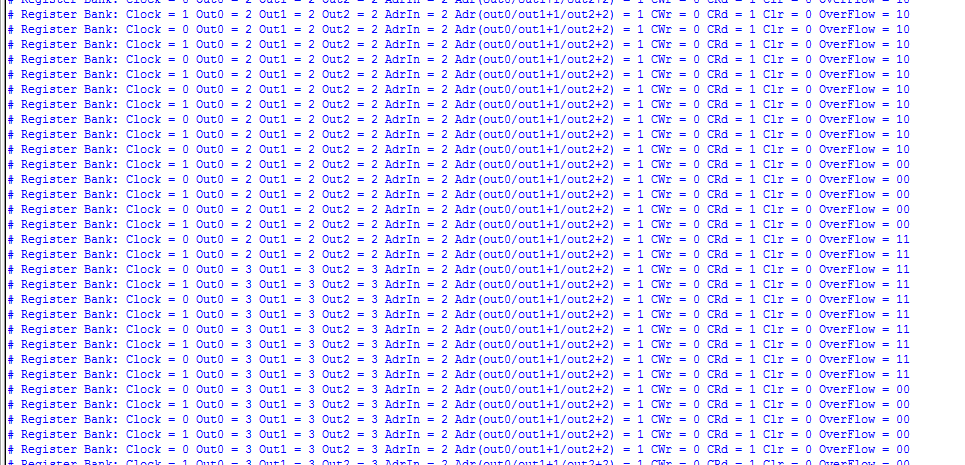
\includegraphics[scale=0.6]{BANKsimu-overflow.PNG}
		\caption{Simulação do banco registradores em casos de overflow, endereço de saida fixo em '1'}
		\label{Rotulo}
	\end{figure}
	Esse caso testa as condições de overflow, fazendo um OR logico com o registrador[1](flg, ou, flag) com o valor de overflow, e funciona corretamente.
	\item Memória\\
	\begin{figure}[H]
		\centering
		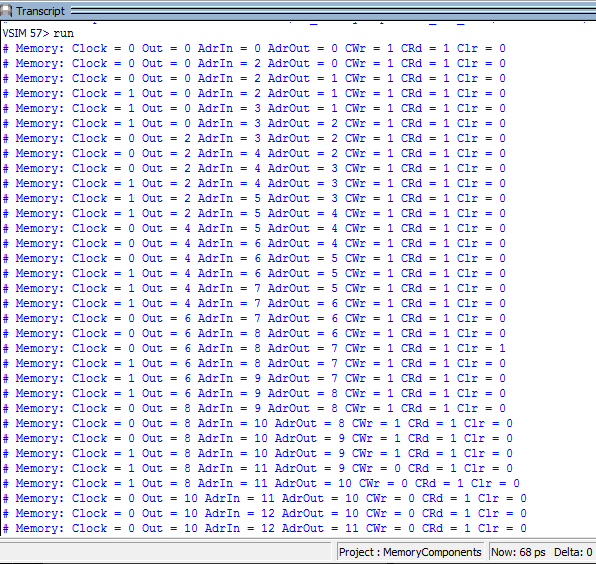
\includegraphics[scale=0.7]{MEMsimu0.PNG}
		\caption{Simulação do da memória}
		\label{Rotulo}
	\end{figure}
	\begin{figure}[H]
		\centering
		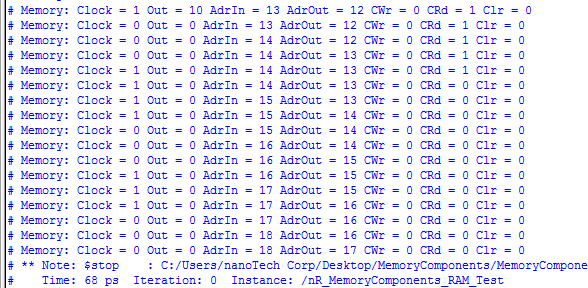
\includegraphics[scale=0.7]{MEMsimu1.PNG}
		\caption{Simulação do da memória}
		\label{Rotulo}
	\end{figure}
	\vfill
	Quando o clock tem borda de subida, o valor no endereco de entradada(que é o mesmo da entrada nesse caso) é gravado, quando temos borda de subida o valor é lido corretamente. Podemos ver tambem que o controle de leitura e escrita tambem funciona, permitindo ou nao leitura e escrita. O sinal assincrono de clear também está funcionado, zerando os valores quando tem nivel logico alto.
\end{itemize}
\newpage
\section{Compilador}
o código do compilador sofreu diversas alterações, o segmento de dados estava sendo interpretado e anexado corretamente, agora, com maior conhecimento sobre o funcionamento do mesmo do mesmo tudo foi corrigido e funciona corretamente. Também foram adicionadas várias flags de compilalção que tem seu funcionamento descrito abaixo:
\subsection{Flags de compilador}
\begin{itemize}
	\item -o\\ Define o nome do arquivo de saída compilado, por padrão o nome é "a.out"
	\item -s\\ Separa a saída em dois arquivos compilados, deixando um arquivo para instruções e outro para dados.
	\item -c\\ Adiciona comentarios no arquivo compilado indicando onde começa cada segmento da memoria
	\item -v\\ Após essa flag é passado o nome da variavél para dados e o nome da variável para instruções, então o compilador gera um código verilog atribuindo a essas variaveis o programa, para simplemente colar no verilog
	\item -b\\ Compila para um arquivo binário
\end{itemize}
\subsection{Novo código do compilador}
\lstinputlisting[language={cpp}]{nanoRiskCompiler.cpp}
\vfill
\section{Controle}
O controle define os bits de controle para cada instrução, abaixo podemos ver o código verilog desse componente, acima do código há um comentario explicando suas entradas e saídas.
\lstinputlisting[language={v}]{Control/Control.v}
\subsection{Simulação}
Para verificar o funcionamento do componente foi criado um código extra para simulações que é o código abaixo:
\lstinputlisting[language={v}]{Control/Control_Test.v}
\subsubsection{Resultados}
O controle simplesmente obedece a tabela de bits de controle atualizando seus valores na borda de subida do clock e seu funcionamento pode ser observado abaixo:
\begin{figure}[H]
	\centering
	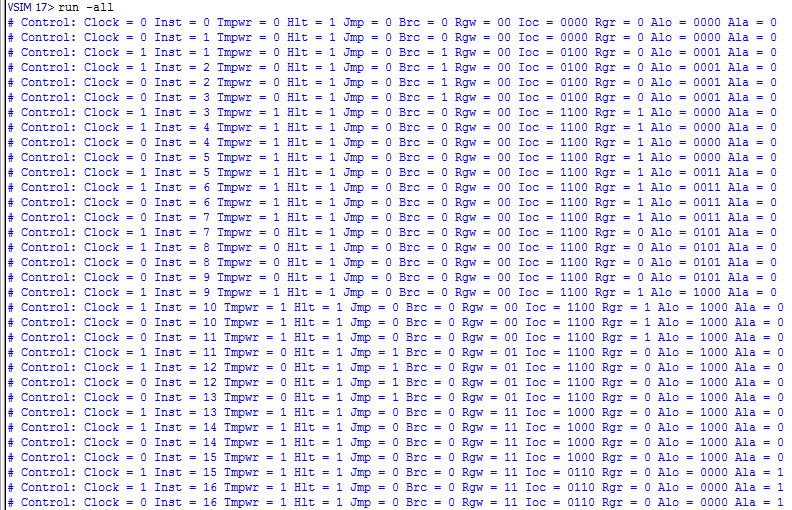
\includegraphics[scale=0.7]{simuCTRL.PNG}
	\caption{Simulação módulo de controle}
	\label{Rotulo}
\end{figure}

\section{ALU}
O ALU ou ULA faz as operações lógicas e aritméticas do processador, abaixo podemos ver o código verilog desse componente, acima do código há um comentário explicando suas entradas e saídas.
\lstinputlisting[language={v}]{ALU/ALU.v}
\subsection{Simulação}
Para verificar o funcionamento do componente foi criado um código extra para simulações que é o código abaixo:
\lstinputlisting[language={v}]{ALU/ALU_Test.v}
\subsubsection{Resultados}
A ULA funciona de forma assíncrona, então devemos observar apenas as entradas e o código de cada operação, para essa simulação foram testadas todas as possibilidades de operações, porém so algumas serão mostradas. É facilmente visível que o módulo está funcional. A imagens das simulações estão abaixo.
\begin{figure}[H]
	\centering
	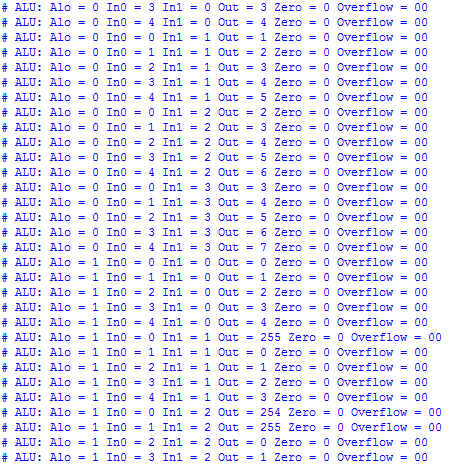
\includegraphics[scale=0.7]{sumuALU(add-sub).PNG}
	\caption{Simulação ALU, operação de soma e subtração}
	\label{Rotulo}
\end{figure}

\begin{figure}[H]
	\centering
	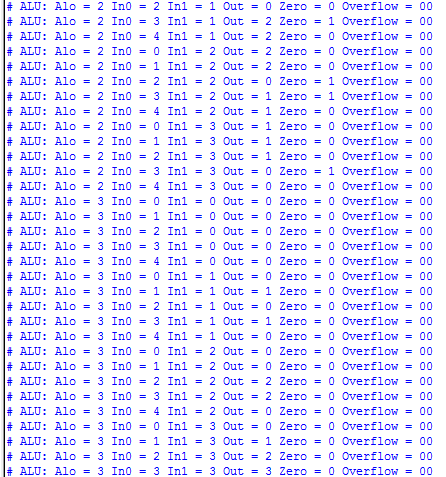
\includegraphics[scale=0.7]{sumuALU(flag-and).PNG}
	\caption{Simulação ALU, operação de flag e and}
	\label{Rotulo}
\end{figure}

\begin{figure}[H]
	\centering
	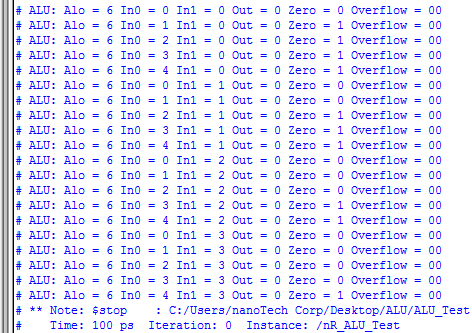
\includegraphics[scale=0.7]{sumuALU(less).PNG}
	\caption{Simulação ALU, operação de less}
	\label{Rotulo}
\end{figure}

\begin{figure}[H]
	\centering
	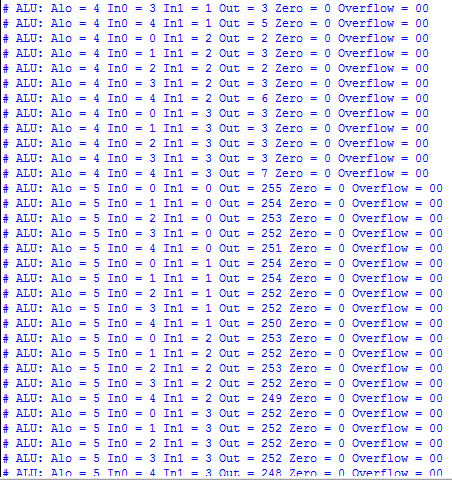
\includegraphics[scale=0.7]{sumuALU(or-nor).PNG}
	\caption{Simulação ALU, operação de or e nor}
	\label{Rotulo}
\end{figure}

\begin{figure}[H]
	\centering
	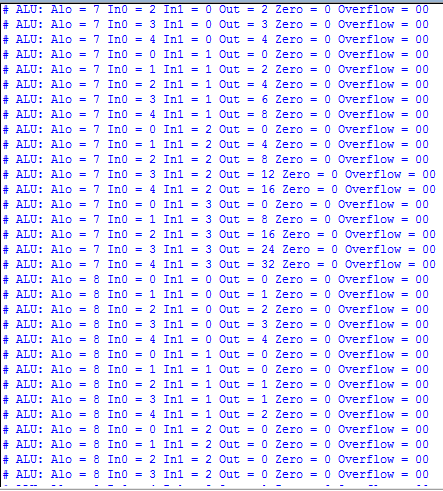
\includegraphics[scale=0.7]{sumuALU(sl-sr).PNG}
	\caption{Simulação ALU, operação de shift esquerda e direita}
	\label{Rotulo}
\end{figure}
A imagem abaixo contem a simulação do modulo somador, que adiciona 1 ou 0 ao endereço de next. A saída é a soma das entradas, seu funcionamento está correto.

\begin{figure}[H]
	\centering
	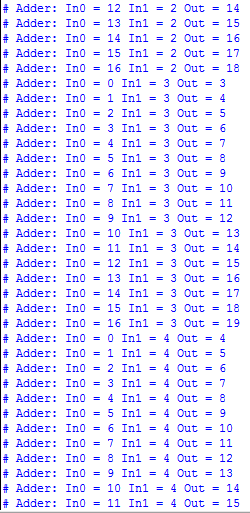
\includegraphics[scale=0.7]{simuAdder.PNG}
	\caption{Simulação módulo de soma}
	\label{Rotulo}
\end{figure}
\newpage
\section{Código compilado}
O código do programa compilado para nanoRisk com a novas alterações do compilador é o código abaixo, espera-se que ele não sofra mais alterações
\lstinputlisting{compiled_commented.txt}
\section{Multiplexador}
Há no projeto multiplexadores de 2 e de 4 entradas.
Os multiplexadores são importantes pois trabalham junto com o controle para definir o caminho dos dados, abaixo podemos ver o código verilog desse componente, acima do código há um comentario explicando suas entradas e saídas.
\lstinputlisting[language={v}]{Miscellaneous/MUX.v}
\subsection{Simulação}
Para verificar o funcionamento do componente foi criado um código extra para simulações que é o código abaixo:
\lstinputlisting[language={v}]{Miscellaneous/MUX_Test.v}
\subsubsection{Resultados}
É possível verificar seu funcionando comparando a simulação abaixo com a tabela da verdade de um MUX.
\begin{figure}[H]
	\centering
	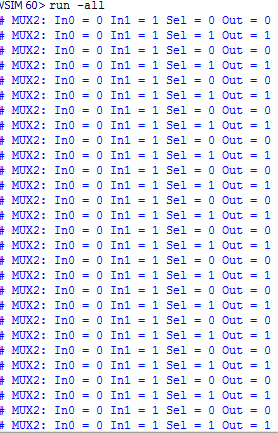
\includegraphics[scale=0.7]{simuMUX2.PNG}
	\caption{Simulação MUX duas entradas}
	\label{Rotulo}
\end{figure}
\begin{figure}[H]
	\centering
	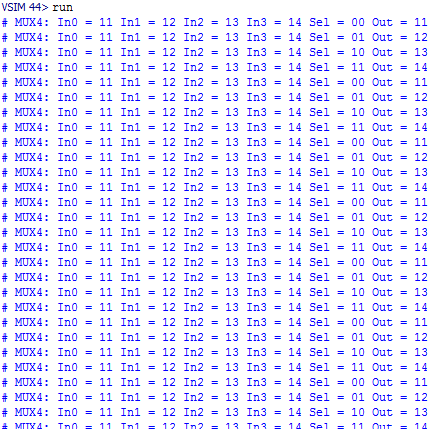
\includegraphics[scale=0.7]{simuMUX4.PNG}
	\caption{Simulação MUX quatro entradas}
	\label{Rotulo}
\end{figure}
\section{Portas lógicas e controle de fluxo}
A portas lógicas usadas são: NOT, AND(2 entradas) e OR(4 entradas), além do controle de fluxo que é uma OR de duas entradas. O código desses componentes está abaixo.
\lstinputlisting[language={v}]{Miscellaneous/Gates.v}
\subsection{Simulação}
Por serem portas lógicas, a simulação escolhida foi por ondas, que é mais simples e de fácil visualização.
\subsubsection{Resultados}
Os resultados das simulações está abaixo e condizem com os resultados esperados.
\begin{figure}[H]
	\centering
	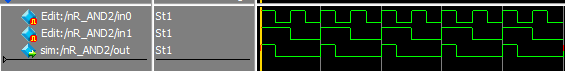
\includegraphics[scale=0.7]{simuAND2.PNG}
	\caption{Simulação AND duas entradas}
	\label{Rotulo}
\end{figure}
\begin{figure}[H]
	\centering
	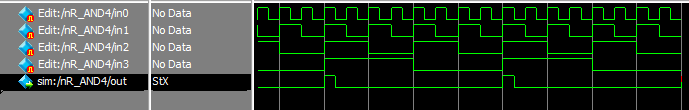
\includegraphics[scale=0.7]{simuAND4.PNG}
	\caption{Simulação porta AND quatro entradas}
	\label{Rotulo}
\end{figure}
\begin{figure}[H]
	\centering
	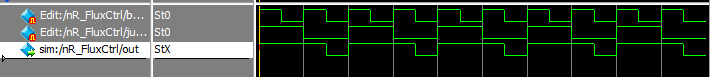
\includegraphics[scale=0.7]{simuFLUXCTRL.PNG}
	\caption{Simulação módulo de controle de fluxo}
	\label{Rotulo}
\end{figure}
\begin{figure}[H]
	\centering
	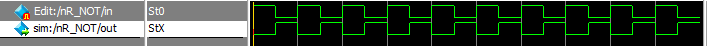
\includegraphics[scale=0.7]{simuNOT.PNG}
	\caption{Simulação porta NOT}
	\label{Rotulo}
\end{figure}
\begin{figure}[H]
	\centering
	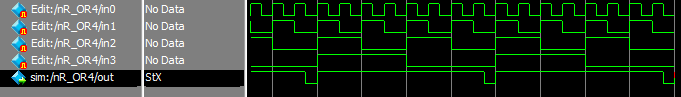
\includegraphics[scale=0.7]{simuOR4.PNG}
	\caption{Simulação porta OR quatro entradas}
	\label{Rotulo}
\end{figure}
\section{BitCmp \& BitExt}
No projeto o BitExt é de 4 para 8 e o BitCmp é de 8 para 1.
Esses componentes ligam vias de diferentes larguras, o BitExt coloca zeros não significativos na entrada e o BitCmp compacta os bits fazendo operações OR entre eles.
\lstinputlisting[language={v}]{Miscellaneous/BitConectors.v}
\subsection{Simulação}
Por ser mais simples, a simulação escolhida foi por ondas, que é mais simples e de fácil visualização.
\subsubsection{Resultados}
Os resultados foram o esperado.
\begin{figure}[H]
	\centering
	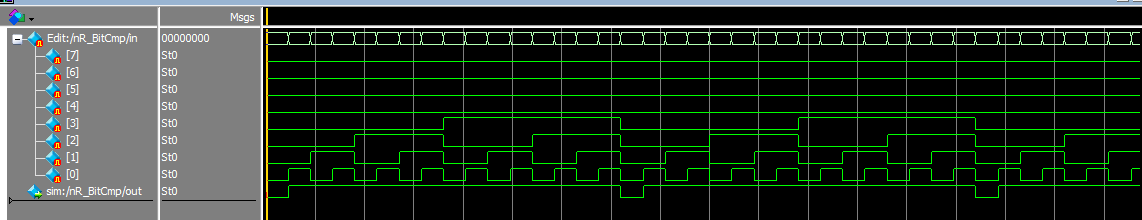
\includegraphics[scale=0.7]{simuCMP.PNG}
	\caption{Simulação compactador de bits}
	\label{Rotulo}
\end{figure}
\begin{figure}[H]
	\centering
	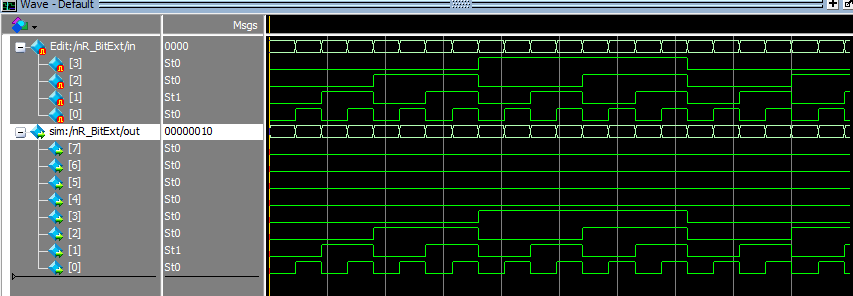
\includegraphics[scale=0.7]{simuEXT.PNG}
	\caption{Simulação extensor de bits}
	\label{Rotulo}
\end{figure}
\section{Correções}
Algumas modificações e adições foram feitas no código do nanoRisk.
\subsection{Nova Porta lógica}
foi feita uma nova porta lógica AND, essa com largura de entrada e saída de 8 bits, ela não foi feita antes devido a uma falta de atenção, se viu necessário o uso dela no caminho de dados. O código dessa porta está abaixo:
\lstinputlisting[language={v}]{novaAnd.v}
\subsection{Alteração no código de Memória}
O código de memória foi alterado também para evitar problemas futuros, na inicialização ele, agora define como zero a saída mas não zera todos os espaços de memória como fazia antes. Com as alterações o novo código é:
\lstinputlisting[language={v}]{novaMemory.v}
\subsection{Alteração no código do Extensor de Bits}
O código do extensor de bits não estava compilando em todos os computadores/versões do modelSIM, por isso, foram feitas alterações na sintaxe do código para deixar tudo mais explicito evitando erros. A lógica manteve a mesma, o novo código é:
\lstinputlisting[language={v}]{novoBitExt.v}
\section{Código do Processador}
O código do processador é a união de todos os componentes até então desenvolvidos seguindo os moldes do diagrama do processador. 
\lstinputlisting[language={v}]{nanoRiskProcessor/nRProcessor.v}
\subsection{Módulo de Teste}
Para testar o processador foi feito um módulo de teste que é apenas uma instanciação do processador que lê o banco de registradores na posição da resposta final para verificar o resultado, o código desenvolvido foi:
\lstinputlisting[language={v}]{nanoRiskProcessor/nRProcessor_Test.v}
\subsection{Simulação}
Durante a simulação se obteve na resposta o número 0 e as vezes 20, quando deveria ser 7. E analisando em tempo real a execução da simulação foi possível ver que alguns componentes funcionavam e outro não, aparentando ser um problema de sincronia ou clock.
\clearpage
\section{Versão 2}
\subsection{Compilador}
\lstinputlisting[language={cpp}]{2/nanoRiskCompiler.cpp}
\subsection{Software}
\lstinputlisting[language={[nanoRisk]Assembler}]{2/software.asm}
\subsection{Hardware}
\lstinputlisting[language={v}]{2/nanoRiskProcessor2.v}

\section{Conclusões} 
Por mais que houvessem limitações no hardware que deve ser proposto foi possível projetar muita coisa e ainda tem espaço para projetar, definir, melhorar muito. A maior limitação é a quantidade de bits, que por mais que facilite na hora da elaboração do hardware vem com muitos problemas, como por exemplo, o maior valor armazenável com 8 bits que é 256, sendo que o problema proposto possui números maiores, a solução então será usar double words(palavras duplas) e tratamento de overflow, este por sua vez não foi efetivo em sua implementação causando vários problemas, não funcionando como o esperado e limitando palavras duplas à números positivos. Foi definido duas flags de overflow para que o programador pudesse trabalhar mais facilmente com numeros unsigned sem que houvesse necessidade de operações especificas para isso. A quantidade menor de registradores também complica um pouco.

Na definição da prática há restrição de não haver entradas nem saídas, porém caso haja tempo e seja aprovado, é possível adicionar entradas e saidas no projeto, já foi definida estrutura para isso através de flags e dos registradores de função(arg e return). É importante lembrar que primeiro de tudo será desenvolvido o projeto como foi proposto, para usar entradas e saídas seria necessário modificar o programa para esperar as leituras e adicionar no hardware essa função. Além disso não foi necessário modificar, as instruções ou estruturas definidas originalmente para colocar conceitos de entrada e saida. O mais interessante desse conceito além de ampliar a interação e aplicação é por exemplo a possibilidade de fazer um outro programa no futuro que funcionaria como um sistema operacional para gravar programas extras na memoria e alternar entre eles, algo que não seria tão complicado devido a simplicidade do projeto.

Tudo que foi proposto está sujeito a modificações na hora de implementar, mas o conceito original será mantido, por exemplo, o registrador base pointer \$bp pode não ser necessário na hora de criar o hardware ou outro registrador pode ser necessário, ou,  a mémoria RAM pode ser dividida ou não, ou, definição de flags e interrupts. 

Foram achados diversos erros no compilador e na lógica do projeto, as instruções lc e la fazem a mesma coisa, faz falta uma instrução de link e o registrador temporário não deveria ser indexado pois o seu uso no software pode causar vários problemas.

Não foi possível ver o projeto funcionando na versão 1, por causa de diversos erros. Uma falha de sincronismo entre os componentes e erros na detecção de bordas do clock podem estar acontecendo além de erros de projeto e implementação.

Entretanto foi desenvolvida uma versão 2 do mesmo projeto em verilog de forma mais intuitiva, sem os circuitos para minimizar variáveis e corrigir erros de projeto e implementação, essa versão foi bem sucedida e é possível observar seu funcionamento na imagem abaixo. Mesmo com as falhas muito foi aprendido durante o desenvolvimento, implementação e correção do projeto sobre projetos, processadores, organização, testes, programação, etc.

\begin{figure}[H]
	\centering
	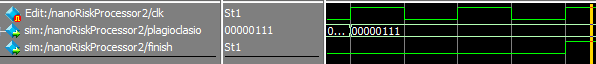
\includegraphics[scale=0.7]{Working.PNG}
	\caption{Simulação do nanoRisk Processor 2}
	\label{Rotulo}
\end{figure}



\end{document}